%=======================================================================================================
%   Fourth-order Multigrid for Overlapping Grids.
%=======================================================================================================
\documentclass{article}
% \usepackage[bookmarks=true]{hyperref} 
\usepackage[bookmarks=true,colorlinks=true,linkcolor=blue]{hyperref}

% \documentclass[xcolor=rgb,svgnames,dvipsnames,11pt]{article}
% \usepackage[bookmarks=true,colorlinks=true,linkcolor=blue]{hyperref}


% \input documentationPageSize.tex
\hbadness=10000 
\sloppy \hfuzz=30pt

% \voffset=-.25truein
% \hoffset=-1.25truein
% \setlength{\textwidth}{7in}      % page width
% \setlength{\textheight}{9.5in}    % page height

\usepackage{calc}
\usepackage[lmargin=.75in,rmargin=.75in,tmargin=.75in,bmargin=.75in]{geometry}


\input homeHenshaw

\usepackage{amsmath}
\usepackage{amssymb}

\usepackage{verbatim}
\usepackage{moreverb}
\usepackage{graphics}    
\usepackage{epsfig}    
% \usepackage{calc}
% \usepackage{ifthen}
% \usepackage{float}
% \usepackage{fancybox}

\usepackage{makeidx} % index
\makeindex
\newcommand{\Index}[1]{#1\index{#1}}

\usepackage{tikz}
\input trimFig.tex

% *** See http://www.eng.cam.ac.uk/help/tpl/textprocessing/squeeze.html
% By default, LaTeX doesn't like to fill more than 0.7 of a text page with tables and graphics, nor does it like too many figures per page. This behaviour can be changed by placing lines like the following before \begin{document}

\renewcommand\floatpagefraction{.9}
\renewcommand\topfraction{.9}
\renewcommand\bottomfraction{.9}
\renewcommand\textfraction{.1}   
\setcounter{totalnumber}{50}
\setcounter{topnumber}{50}
\setcounter{bottomnumber}{50}

\newcommand{\red}{\color{red}}
\newcommand{\green}{\color{green}}

\begin{document}

% -----definitions-----

\newcommand{\ogen}{/home/henshaw/res/ogen}
\newcommand{\figures}{/home/henshaw/Overture/docFigures}
\newcommand{\automg}{/home/henshaw/papers/automg}
% \newcommand{\automg}{../automg}
\newcommand{\ogmgDir}{/home/henshaw/Overture/ogmg}
% \newcommand{\ogmgDir}{.}

\newcommand{\Ogen}{{Ogen}}
\newcommand{\Overture}{{Overture}}
\newcommand{\Ogmg}{{Ogmg}}
\newcommand{\figWidth}{.495\linewidth}
\newcommand{\clipfig}{}
\newcommand{\tablefontsize}{\normalsize}

\input wdhDefinitions.tex


%--------------------- TITLE PAGE -------------------------------
\vglue 10\baselineskip
\begin{flushleft}
{\Large
A Fourth-order Accurate Multigrid Solver for Overlapping Grids \\
}
\vspace{2\baselineskip}
William D. Henshaw  \\
Department of Mathematical Sciences, \\
Rensselaer Polytechnic Institute, \\
Troy, NY, USA, 12180.
\vspace{\baselineskip}
\today\\
\vspace{\baselineskip}

\vspace{4\baselineskip}

% --------------------------- ABSTRACT -----------------------------------
\noindent{\bf Abstract:}
  
  An algorithm is described for the fourth-order accurate solution of elliptic boundary
value problems on overlapping grids using the multigrid algorithm. The
fourth-order accurate discretization, with a stencil 5 points wide in each
direction, is solved directly with multigrid. The automatic grid coarsening algorithm
described in~\cite{OnMultigrid} is extended to the fourth-order accurate case, allowing the
generation of very coarse grids.
%
The discretization of the partial differential equation on the
coarse grid can be generated automatically from the fine grid discretization
using Galerkin averaging.
%
A good approach for choosing numerical boundary conditions for Dirichlet and Neumann/mixed
boundary conditions is described. By using the partial differential equation, 
numerical boundary conditions
can be derived which are consistent with the eigen-structure of the problem.
The resulting scheme shows no degradation of convergence rates for Dirichlet or Neumann/mixed
boundary conditions.
%
The smoothing rates of Red-Black smoothers for the fourth-order discretization
can be significantly improved through
the use of an over-relaxation parameter and we determine the appropriate values
for this parameter.
%
Numerical results are presented showing that very good multigrid convergence rates can be obtained. 
The rates for the fourth-order approximations are often nearly as
good as those for second-order discretizations. 
Furthermore, the time required for the solution of a fourth-order accurate discretization 
is often only about $50\%$ greater than a comparable second-order accurate solution.

\end{flushleft}

\vfill\eject
\tableofcontents
% \listoffigures

%---------- End of title Page for a Research Report


\vfill\eject
\section{Introduction}\index{multigrid}


  An algorithm is described for the fourth-order accurate solution of elliptic boundary
value problems on overlapping grids using the multigrid algorithm. The
fourth-order accurate discretization, with a stencil 5 points wide in each
direction, is solved directly with multigrid. The automatic grid coarsening algorithm
described in~\cite{OnMultigrid} is extended to the fourth-order accurate case, allowing the
generation of very coarse grids.
%
The discretization of the partial differential equation on the
coarse grid can be generated automatically from the fine grid discretization
using Galerkin averaging.
%
A good approach for choosing numerical boundary conditions for Dirichlet and Neumann/mixed
boundary conditions is described. By using the partial differential equation, 
numerical boundary conditions
can be derived which are consistent with the eigen-structure of the problem.
The resulting scheme shows no degradation of convergence rates for Dirichlet or Neumann/mixed
boundary conditions.
%
The smoothing rates of Red-Black smoothers for the fourth-order discretization
can be significantly improved through
the use of an over-relaxation parameter and we determine the appropriate values
for this parameter.
%
Numerical results are presented showing that very good multigrid convergence rates can be obtained. 
The rates for the fourth-order approximations are often nearly as
good as those for second-order discretizations. 
Furthermore, the time required for the solution of a fourth-order accurate discretization 
is often only about $50\%$ greater than a comparable second-order accurate solution.

\section{Fourth-order accurate discretization on overlapping grids}

Consider solving an elliptic boundary value problem in $d=2,3$ space dimensions,
\begin{align*}
  L u & = f \qquad \xv\in\Omega \\
  B u & = g \qquad \xv\in\partial\Omega
\end{align*}
where $L$ is an elliptic operator, $B$ the boundary operator and $\xv=(x_1,x_2,\ldots,x_d)\in \Real^d$.
We will also use the notation $\xv=(x,y,z)$, when convenient.

\newcommand{\ct}{\tilde{c}}
\newcommand{\alphat}{\tilde{\alpha}}
In this paper we take $L$ to be a second-order linear variable coefficient operator
and $B$ to define a Dirichlet, Neumann or mixed boundary condition. In two space dimensions these would
take the form
\begin{align}
   L u &:= \ct_{11} u_{xx} + \ct_{12} u_{xy} + \ct_{22} u_{yy} 
                     + \ct_1 u_x + \ct_2 u_y + \ct_0 u = f \label{eq:cts-pde} \\
%   Lu &= \sum_{m,n=0}^d 
%           \ct_{m_1 m_2 m_3} \partial_{x_1}^{m_1}\partial_{x_2}^{m_2}\partial_{x_3}^{m_3}   u  \label{eq:cts-pde} \\
%      &= \ct_{200} \partial_x^2 u + \ct_{110} \partial_x\partial_y u + \ct_{020} \partial_y^2 + \ldots
%            + \ct_{100} \partial_x u +\ldots \ct_{000} u  \\
   Bu &= \alphat_1 \partial_n u + \alphat_0 u             \label{eq:cts-bc}
\end{align}
Here $\partial_n u=\nv\cdot\grad u$ is the normal derivative of $u$, with $\nv$ the unit outward
normal to the boundary $\partial\Omega$. The extension to three-dimensions is straight forward.


Intro: $G_g, \xv,\rv, \xv_\iv$

On a given component grid $G_g$ we transform the equations (\ref{eq:cts:pde}-\ref{eq:cts-bc})
to the unit square coordinates $\rv=(r_1,r_2)=(r,s)$,
\begin{align}
    L u &:= c_{11} u_{rr} + c_{12} u_{rs} + c_{22} u_{ss} 
                     + c_1 u_r + c_2 u_s + c_0 u = f \label{eq:cts-pde} \\
   Bu &= \alpha_1 \partial_r u + \alpha_2 \partial_s u + \alpha_0 u             \label{eq:cts-bc-r}
\end{align}
or the conservative form ??

Let $U_\iv$ denote the numerical approximation to $u(\xv_\iv)$.
The equations are discretized to fourth-order accuracy using standard
centred approximations such as
\begin{align} 
  \partial_r &\approx D_{4r} \equiv D_{0r}\Big( 1 - {h^2\over6} D_{+r}D_{-r}\Big) \\
  \partial_r^2 &\approx D_{4rr} \equiv D_{+r}D_{-r}\Big( 1 - {h^2\over12} D_{+r}D_{-r}\Big) \\
  \partial_r\partial_s &\approx D_{4rs} \equiv D_{4r}D_{4s}
\end{align}
where $D_{+r}$, $D_{-r}$, and $D_{0r}$ are the forward backward and central difference operators.


The fourth-order discrete approximation to (\ref{eq:cts:pde-r}-\ref{eq:cts-bc-r})
is given by
\begin{align*}
   L_h U &= c_{11} D_{4rr} U_\iv + c_{12} D_{4rs} U_\iv + c_{22} D_{4ss} U_\iv \ldots
          + c_{1} D_{4r} U_\iv + c_{2} D_{4s} U_\iv + c_{0} U_\iv         \\        
   B_h U &= \alpha_1 D_{4r} U_\iv + \alpha_2 D_{4s} U_\iv + \alpha_0 U_\iv   
\end{align*}
where, for example
\begin{align*}
  c_{11} &=  \ct_{11}~r_x^2 + \ct_{22}~ r_y^2  \\
  c_1    &=   \ct_1~r_x + \ct_2~r_y + \ct_{11}~r_{xx} 
\end{align*}

Consider a problem with a boundary condition at $r_1=0$, $i_1=0$. 
On a boundary with a Dirichlet condition, one ghost line is introduced. 
The discrete equations will be of the form
\begin{align*}
   L_h U_\iv &= f_\iv \qquad i_1=1,2,3,\ldots \\
      U_\iv & = g_\iv   \qquad i_1=0 \\
      B^{(D)} U_\iv & = g_\iv^{(D)}  \qquad i_1=-1 \qquad\mbox{(numerical boundary condition)}
\end{align*}
On a boundary with a Neumann or mixed condition the interior PDE is applied on the boundary
and two ghost line are introduced.
\begin{align*}
   L_h U_\iv &= f_\iv \qquad i_1=0,1,2,3,\ldots \\
      \alpha_1 D_{4r} U_\iv + \alpha_2 D_{4s} U_\iv + \alpha_0 U_\iv &= g_\iv   \qquad i_1=0 \\
      B^{(N)} U_\iv & = g_\iv^{(N)}  \qquad i_1=-2 \qquad\mbox{(numerical boundary condition)}
\end{align*}
In either case one extra numerical boundary is required to define the discretization.
In the Dirichlet case the numerical boundary condition is considered to define the value of $U_\iv$
at $i_1=-1$, while in the Neumann case it is considered to define the value at $i_1=-2$.

% =================================================================================
\clearpage
\section{Operator averaging}

To generate a coarse grid operator from a fine grid operator we can
average the operator on the fine grid and then restrict the result
to the coarse grid.

Consider a 3 point stencil operator in one dimension. If we look at the stencil for
rows $i-1,i,i+1$ arranged in a matrix then we get
\[
   \begin{matrix}
   a_{i-1}u_{i-2} & b_{i-1}u_{i-1} & c_{i-1} u_i  & 0              & 0 \\
       0          & a_i u_{i-1}    & b_i u_i      & c_i u_{i+1}    & 0\\
       0          &       0        & a_{i+1} u_i  & b_{i+1}u_{i+1} & c_{i+1}u_{i+2} \\
    \end{matrix}
\]
If we replace row $i$ by the weighted average of rows $i-1,i,i+1$ with weights $\alpha$, $\beta$, $\alpha$
then we get the wide stencil
\[
   \begin{matrix}
     \alpha a_{i-1}u_{i-2} & 
         (\alpha b_{i-1}+\beta a_i)u_{i-1}  &
         (\alpha( c_{i-1} + a_{i+1}) + \beta b_i ) u_i &
         (\alpha b_{i+1}+\beta c_i)u_{i-1}  &
     \alpha c_{i+1}u_{i+2} 
    \end{matrix}
\]
If we distribute the values at point $i-1$ using $u_{i-1}=\half( u_{i-2}+u_i )$ and at point $i+1$
using $u_{i+1}=\half( u_{i+2}+u_i )$ then we have a wide stencil only defined at points
$i-2,i,i+2$.
\[
   \begin{matrix}
     ( \alpha(a_{i-1}+\half b_{i-1}) +\half\beta a_i) u_{i-2} & 
         &
         (\alpha( \half b_{i-1} + \half b_{i+1} + c_{i-1} + a_{i+1}) + \beta (b_i+\half a_i+\half c_i) ) u_i &
         &
     (\alpha( c_{i+1}\half b_{i+1}) + \half\beta c_i)u_{i+2} 
    \end{matrix}
\]

Typically we take $\alpha=\gamma=1/4$, and $\beta=1/2$.  In more than one space dimension we can
apply the above averaging procedure sequentially in each direction. 


Now consider a 5 point operator (we could also average 5 adjacent equations rather then 3)
\[
   \begin{matrix}
a_{i-1}u_{i-3}& b_{i-1}u_{i-2}& c_{i-1} u_{i-1}& d_{i-1} u_{i} & e_{i-1} u_{i+1} &  0              & 0 \\
    0         & a_i u_{i-2}   & b_i u_{i-1}    & c_i u_{i  }   & d_{i  } u_{i+1} & e_{i  } u_{i+2} & 0\\
    0         &       0       & a_{i+1} u_{i-1}& b_{i+1}u_{i}  & c_{i+1}u_{i+1}  & d_{i+1} u_{i+2} & e_{i+1} u_{i+3} \\
    \end{matrix}
\]
Averaging in a similar fashion we obtain a coarse grid operator
\[
   \begin{matrix}
    a_i^c u_{i-2}   & b_i^c u_{i-1}    & c_i^c u_{i}  & d_{i}^c u_{i+1} & e_{i}^c u_{i+2} \\
    \end{matrix}
\]
where
\begin{align*}
   a_i^c &= \half\alpha a_{i-1} \\  
   b_i^c &=  \alpha b_{i-1} + \beta a_i + \half \alpha a_{i-1}+
                \half( \alpha c_{i-1} + \beta b_i + \alpha a_{i+1} )      \\
   c_i^c &= \alpha d_{i-1} + \beta c_i +\alpha b_{i+1} +
               \half( \alpha c_{i-1} + \beta b_i + \alpha a_{i+1} ) +
               \half( \alpha e_{i-1} + \beta d_i + \alpha c_{i+1} ) \\
   d_i^c &=  \alpha d_{i+1} + \beta e_i +
              \half( \alpha e_{i-1} + \beta d_i + \alpha c_{i+1} ) +
               \half\alpha e_{i+1} \\
   e_i^c &= \half\alpha e_{i+1} \\  
\end{align*}


\subsection{Operator averaging at boundaries}

   At a boundary we will typically have a boundary condition such as a dirichlet, neumann or mixed boundary
condition. We need to decide how to average near the boundary and on the boundary or ghost line.

Ogmg is aware of two types of boundary conditions. These 'boundary conditions' actually
just indicate how the {\bf ghost line} should be updated. The condition {\tt extrapolation} indicates the 
ghost line is extrapolated and usually means that a dirichlet boundary condition is applied on
the boundary. The {\tt equation} boundary condition indicates that some equation is applied on
the ghost line; this is usually associated with a neumann or mixed boundary condition.

\begin{description}
  \item[dirichlet] : In this case we just impose a dirichlet BC in the coarse grid operator.
  \item[neumann] : (or neumann like condition) coarse grid operator. The coarse grid operator is
     obtained by distributing the fine grid ghost line equation to the coarser grid but not averaged
     in the tangential direction.
\[
   \begin{matrix}
     ( \alpha(a_{i}+\half b_{i}) +\half\beta a_i) u_{i-2} & 
         &
         (\alpha( b_i + c_i + a_i) + \beta (b_i+\half a_i+\half c_i) ) u_i &
         &
     (\alpha( c_i + \half b_i) + \half\beta c_i)u_{i+2} 
    \end{matrix}
\]
  \item[extrapolation] : coarse grid operator is also extrapolation.
  \item[equation] : ghost line has some equation on it. The coarse grid operator is obtained by
       averaging the ghostline equations (i.e. averaging is only done in the tangential directions).
\end{description}






{\bf Remark:} 
The coarse grid matrix $A^{2}$ can also be defined from the fine grid matrix $A^1$ using the prologation
and restriction operators
\[
     A^2 = R A^1 P
\]
The first step above where the rows were combined corresponds to premultiplying $A^1$
by $R$.
The second step where the values at points $i+1$ and $i+1$ were removed corresponds to the post-multiplication
by $P$.

Tables~(\ref{tab:operatorAveraging}-\ref{tab:operatorAveraging4}) 
compare the convergence results for Poisson's equation with 
dirichlet boundary conditions when using operator averaging to construct the coarse grid equations
to no operator averaging. The notation used to label the columns in defined 
at the start of section~\ref{sec:numericalResults}.
In this example the operator-averaged case is significantly better.
There was a negligible difference in CPU times between the two cases.


{
\renewcommand{\figWidth}{6.cm}
\newcommand{\trimfig}[2]{\trimhb{#1}{#2}{.0}{.0}{.0}{.0}}
\begin{figure}[hbt]
\begin{center}
\begin{tikzpicture}[scale=1]
  \useasboundingbox (0,.7) rectangle (15.5,6.5);  % set the bounding box (so we have less surrounding white space)
%
  \draw ( 0.0,0.0) node[anchor=south west,xshift=-4pt,yshift=+0pt] {\trimfig{fig/opAveComparison4}{\figWidth}};
  \draw ( 8.0,0.0) node[anchor=south west,xshift=-4pt,yshift=+0pt] {\trimfig{fig/opAveComparison4-box128}{\figWidth}};
%
 % \draw (current bounding box.south west) rectangle (current bounding box.north east);
% grid:
% \draw[step=1cm,gray] (0,0) grid (15,6);
\end{tikzpicture}
\end{center}
\caption{The convergence rate is improved when the coarse grid operators are generated
with operator averaging. Results are shown for a V[2,1] cycle.}
\label{fig:opAveComparison}
\end{figure}
}

% \renewcommand{\figWidth}{.495\linewidth}
% \begin{figure}
% \begin{center}
% % \epsfig{file=opAveComparison.eps,width=\figWidth}
% 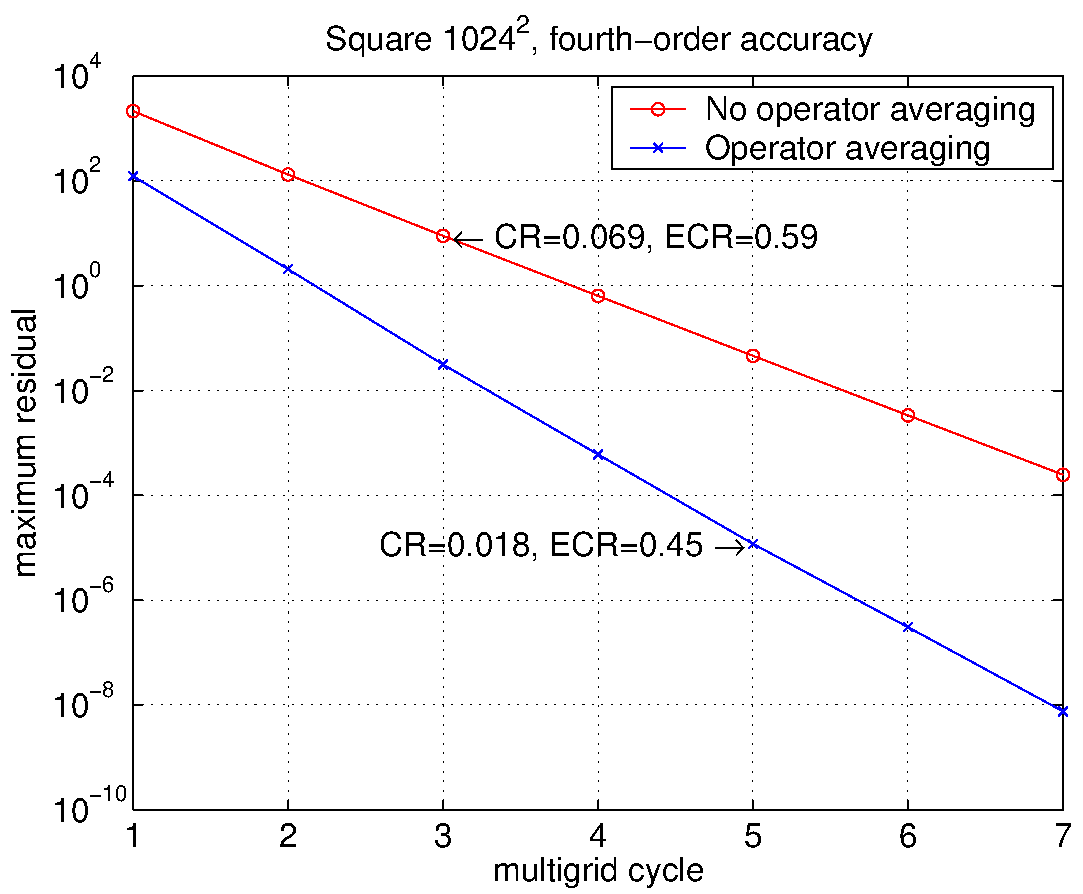
\epsfig{file=opAveComparison4.eps,width=\figWidth}
% % \epsfig{file=opAveComparison.box128.eps,width=\figWidth}
% \epsfig{file=opAveComparison4.box128.eps,width=\figWidth}
% \end{center}
% \caption{The convergence rate is improved when the coarse grid operators are generated
% with operator averaging. Results are shown for a V[2,1] cycle.}
% \label{fig:opAveComparison}
% \end{figure}



% -----------------------------------------------------------
\clearpage
\section{Smoothing overlapping grids}

There are a few issues that must be addressed when smoothing an overlapping grid.
Some care must be taken to ensure that the composite-smooth operator (a smoothing step
over all component grids) retains similiar smoothing rates to that of a smoother for a 
single component grid. The underlying principle for smoothing an overlapping
grid is that the defect after smoothing should be smooth enough to be represented 
on the next coarser levels.

\subsection{IBS: Smoothing near interpolation boundaries}

  The defect can sometimes become large right next to an interpolation boundary. In this section 
we describe why this happens and what can be done to alleviate the problem.
In the last step of the composite-smoothing operator~\ref{compositeSmooth}, an overlapping grid
interpolation operation is performed. It has long been recognised that this last step has the potential
for introducing a non-smooth component to the solution since the solution is not smoothed after
this interpolation. This last step is included since the convergence rates are, in practice,
almost always better when its addition.
The cause of the non-smoothness is illustrated in figure~\ref{fig:compSmoothDisc} for the case
of two grids, $G_1$ and $G_2$. At the final step in the composite smooth the interpolation points
are shifted to match the current solutions. This can cause nearby defects to become large.

If there is a very small overlap (i.e. the overlap is some fraction of a mesh wdith), 
as is typical with second order methods, this is usually not a serious problem. Fourth-order accurate methods
have two lines of interpolation and this the overlap is larger. Figure~\ref{fig:cicDisc} shows the defect for
a circle-in-a channel grid. There is a large defect near the interpolation boundary. This results in 
a serious degradation of the convergence rate from ?? to about ??.

In order to fix this problem we have developed a interpolation-boundary-smoothing procedure, IBS,  as outlined in the
algorithm given in figure~(\ref{alg:smoothInterp}).


Typical values for a fourth-order accurate problem are $n_I=2$, $m_I=2$, and $w_I=4$. 
These values would mean that for each of $n_I=2$ global iterations we
smooth $w_I=4$ layers of discretization points near interpolation points with $m_I=2$ sub-iterations of Gauss-Seidel.

Figure~\ref{fig:smoothInterp} shows an example where smoothing near the interpolation boundaries
can significantly improve the convergence rate. With the addition of the IBS procedure the convergence rate
is almost optimal in the sense that it is basically the same as that obtained for a single square grid.

{
\renewcommand{\figWidth}{6.cm}
\newcommand{\trimfig}[2]{\trimhb{#1}{#2}{.0}{.0}{.0}{.0}}
\begin{figure}[hbt]
\begin{center}
\begin{tikzpicture}[scale=1]
  \useasboundingbox (0,.7) rectangle (15.,6.5);  % set the bounding box (so we have less surrounding white space)
%
  \draw ( 0.0,0.0) node[anchor=south west,xshift=-4pt,yshift=+0pt] {\trimfig{fig/interpSmoothing-cic3-order4}{\figWidth}};
%
 % \draw (current bounding box.south west) rectangle (current bounding box.north east);
% grid:
% \draw[step=1cm,gray] (0,0) grid (15,6);
\end{tikzpicture}
\end{center}
\caption{A comparison showing the benefit of using interpolation boundary smoothing (IBS)
 for a circle-in-a-channel, fourth-order accurate, W[2,1], cic3.order4.}
\label{fig:smoothInterp}
\end{figure}
}

%\begin{figure}[hbt]
%\begin{center}
%\vglue-.125in
%\epsfig{file=interpSmoothing.cic3.order4.eps,width=\figWidth}
%\end{center}
%\caption{A comparison showing the benefit of using interpolation boundary smoothing (IBS)
% for a circle-in-a-channel, fourth-order accurate, W[2,1], cic3.order4.}
%\label{fig:smoothInterp}
%\end{figure}




% ****************************************************************************************
\clearpage
\section{Smoothers}

  A variety of smoothers are available for use with Ogmg. These include
\begin{description}
  \item[Red-Black:] $\omega$-RB-GS - Red-Black Gauss-Seidel with a relaxation coefficient $\omega$,
     is generally the
     best smoother for the Laplace operator on grids that are not too highly stretched.
  \item[Jacobi:] $\omega$-Jac - under-relaxed Jacobi is a reasonable smoother. It gives a much smoother
     looking and symmetric defect than $\omega$-RB-GS and so can be useful for debugging.
  \item[Gauss-Seidel:] $\omega$-GS. 
  \item[Line-Jacobi:] $\omega$-xLJac, $\omega$-yLJac, $\omega$-zLJac, $\omega$-aLJac
  \item[Line-Zebra:] $\omega$-xZGS, $\omega$-yZGS, $\omega$-zZGS,$ \omega$-aZGS, - 
    $x,y,z$ and alternating line-zebra are often the best smoothers 
    for highly stretched grids. In three dimensions it pays to include a relaxation coefficient, $\omega$.
\end{description}




% ==============================================================================================================

\newcommand{\thetav}{\boldsymbol{\theta}}

\subsection{Smoothing Factors}

   The smoothing rate of Red-Black smoothers can be significantly improved through
over-relaxation. 
The effect is more pronounced in three-dimensions,
for fourth-order discretizations and for stretched grids.
For second-order methods, the proper choice of $\omega$ was derived by Yavneh~\cite{Yavneh96}. 
Here we extend Yavneh's results to fourth-order discretizations.

% The choice of relaxation parameters for Jacobi and red-Black smoothers is now


We will use local-fourier-analysis (LFA) (also known as normal-mode-analysis)
to determine the smoothing properties
of relaxed Jacobi ($\omega$-Jacobi) and relaxed Red-Black-Gauss-Seidel ($\omega$-RB-GS) smoothers.
We begin with $\omega$-Jacobi since the analysis is more straight-forward. See Trottenberg et.al.~\cite{Trottenberg2001}
for further details on LFA.

Consider the solution to the Poisson equation in $d=2$ or $d=3$ space dimensions,
\[
     L u := \sum_{m=1}^d c_m \partial_{x_m}^2 u  = f
\]
on the periodic unit square. 
We assume that $c_m>0$ and that the operator has been scaled so that
$\sum_m c_m =1$.
Consider the standard second-order discrete approximation to $L$, 
\[
   L_h = \sum_m c_m D_{+x_m}D_{-x_m} 
\]
where we assume equal grid spacing $h$ in each direction (this can always be achieved by rescaling
the coefficients $c_m$).

Let
\[ 
    L_h = D + C
\]
be a splitting of $L_h$ into the diagonal part and the rest.
The Jacobi relaxation scheme is given by 
\[
   D w_{\iv}^{n+1} = -C w_{\iv}^{n}
\]
or
\begin{align*}
    w_{\iv}^{n+1} & = - D^{-1}C w_{\iv}^{n} \\
                  &= (I - D^{-1}( D+C ) )w_{\iv}^{n} \\
                  &= (I - D^{-1}L_h )w_{\iv}^{n}
\end{align*}
The $\omega$-Jacobi relaxation scheme is
\[
   w_{\iv}^{n+1} =  (I - \omega D^{-1} L_h ) w_{\iv}^{n}
\]
Local-fourier-analysis  proceeds by 
looking for a solution of the form
\begin{align*}
   w_{\iv}^{n} &= \alpha^n \exp^{ i \thetav\cdot\xv/\hv }  \\
               &= \alpha^n \exp^{ i (\theta_1 x_1/h_1 + \ldots \theta_d x_d/h_d) }
\end{align*}
where $\thetav=(\theta_1,\ldots,\theta_d)$. Susbtitution into the $\omega$-Jacobi smoothing
operator  gives 
\begin{align*}
    \alpha &= \hat{S}_h(\omega)  \\
           &= 1 - \omega ( 1 - \sum_m c_m \cos(\theta_m) )
\end{align*}
where $\hat{S}_h(\omega)$ is called the symbol of the operator.
The smooth modes correspond to 
\[
 \thetav\in \Theta^{(s)} = [-\pi/2,\pi/2]^d \qquad\mbox{(smooth frequencies)}
\]
while the rough modes correspond to the frequencies that remain,
\[
\Theta^{(r)} = [-\pi,\pi]^d - \Theta^{(s)} \qquad\mbox{(rough frequencies)}
\]

\newcommand{\cmin}{c_{\rm min}}
\newcommand{\cmax}{C_{\rm max}}

The smoothing factor $\mu_{\rm loc}(\omega)$ is defined to be
\[
   \mu_{\rm loc} (\omega) = \sup_{h>0} \sup_{\thetav\in \Theta^{(r)}} \vert  \hat{S}_h(\omega)  \vert
\]
Now for $\thetav\in \Theta^{(r)}$
\begin{align*}
     \hat{S}_h((-\pi,\ldots,-\pi) &\le \hat{S}_h(\omega) \le
            \max \{ \hat{S}_h((\pi/2,0,0),\hat{S}_h((0,\pi/2,0), \hat{S}_h((0,0,\pi/2) \} \\
      1-2\omega &\le \hat{S}_h(\omega) \le 1 - \cmin \omega 
\end{align*}
where $\cmin = \min_m c_m$.
Thus
\[
    \mu_{\rm loc}(\omega) =  \max( \vert 1 - \cmin\omega \vert, \vert 1 - 2\omega \vert )
\]
The best smoothing rate occurs for 
\begin{align*}
  \omega_{\rm opt} &= {1\over 1+ \cmin/2} \qquad\mbox{($\omega$-Jac)}\\
 \mu_{\rm loc}(\omega_{\rm opt}) &= {1 - \cmin/2 \over 1+ \cmin/2 } \qquad\mbox{($\omega$-Jac)}
\end{align*}
In particular, for the 2D Laplace operator, $c_1=c_2=1/2$ and $\omega_{\rm opt}=4/5$, $\mu_{\rm loc}=3/5$
while in 3D, $c_1=c_2=c_3=1/3$ and $\omega_{\rm opt}=6/7$, $\mu_{\rm loc}=5/7$.
Note that on a stretched or curvilinear grid one may choose a different value of $\omega$ at each grid point based
on the local value of $\cmin$.

Now consider the fourth-order accurate discretization,
\[
   L_h^{(4)} = \sum_m c_m D_{+x_m}D_{-x_m}\Big( 1 - {h^2\over12} D_{+x_m}D_{-x_m} \Big)
\]
with symbol
\begin{align*}
  \hat{L}_h^{(4)}(\thetav) &= {1\over 6 h^2}\Big[ -15 + 16 C(\thetav) - C(2\thetav) \Big],
\end{align*}  
where 
\begin{align*}
  C(\thetav) &=\sum_m c_m\cos(\theta_m) 
\end{align*}  
The symbol of the $\omega$-Jacobi smoothing operator is
\begin{align*}
    \hat{S}_h^{(4)}(\omega)  &= 1 - \omega \Big[ 1 - {16\over15}C(\thetav) + {1\over 15}C(2\thetav) \Big] \\
    \hat{S}_h^{(4)}(\omega)  &= 1 - \omega \Big[ 1 - C_4(\theta)  \Big]
\end{align*} 
where
\begin{align*}
     C_4(\theta) &= {16\over15}C(\thetav) - {1\over 15}C(2\thetav) \\
                 &= (1+\beta)C(\thetav) - \beta C(2\thetav)
\end{align*}   
with $\beta=1/15$. By setting $\beta=0$ the results should reduce to those of the second-order case.
Now (*prove this*) sharp bounds on $C_4(\thetav)$ are
\begin{align*}
      -(1+2\beta) \le C_4(\thetav) &\le 1 - (1-\beta) \cmin \qquad\mbox{for $\thetav\in\Theta^{(r)}$} \\
    C_4(\pi,\ldots,\pi)& =  -(1+2\beta) \\
    \max \{ C_4(\pi/2,0,0),\ldots,C(0,0,\pi/2) \}  &= 1 - (1-\beta) \cmin
\end{align*} 
and thus sharp bounds on $hat{S}_h^{(4)}$ are
\[
  1 - {(2+2\beta)} \omega  \le  \hat{S}_h^{(4)}(\omega) \le 1 - {(1-\beta)}\cmin\omega \qquad\mbox{for $\thetav\in\Theta^{(r)}$}
%   1 - {32\over15} \omega  \le  \hat{S}_h^{(4)}(\omega) \le 1 - {14\over 15}\cmin\omega \qquad\mbox{for $\thetav\in\Theta^{(r)}$}
\]
The smoothing factor $\mu_{\rm loc}^{(4)}(\omega)$ is 
\[
   \mu_{\rm loc} (\omega) = \max(\vert 1 - {(2+2\beta)} \omega\vert, \vert 1 - {(1-\beta)}\cmin\omega \vert )
%   \mu_{\rm loc} (\omega) = \max(\vert 1 - {32\over15} \omega\vert, \vert 1 + {16\over 15}\cmin\omega \vert )
\]
The best smoothing rate occurs for *** finish ***
\begin{align*}
  \omega_{\rm opt} &= {1\over 1+\beta+ (1-\beta)\cmin/2} \qquad\mbox{($\omega$-Jac(4))}\\
 \mu_{\rm loc}(\omega_{\rm opt}) &= { 1+\beta- (1-\beta)\cmin/2 \over 1+\beta+ (1-\beta)\cmin/2} \qquad\mbox{($\omega$-Jac(4))}
%  \omega_{\rm opt} &= {1\over {16\over15} + {7\over15}\cmin} \qquad\mbox{($\omega$-Jac(4))}\\
% \mu_{\rm loc}(\omega_{\rm opt}) &= {1 - {7\over16}\cmin \over 1+ {7\over16}\cmin} \qquad\mbox{($\omega$-Jac(4))}
\end{align*}
In particular, for the 2D Laplace operator, $c_1=c_2=1/2$,  and
\begin{align*}
 \omega_{\rm opt} & =4/(5+\beta)  \qquad \mbox{$\omega$-Jacobi(4), 2D)} \\
  \mu_{\rm loc} & =(3+5\beta)/(5+3\beta) \qquad \mbox{$\omega$-Jacobi(4), 2D)}
\end{align*}
while in 3D, $c_1=c_2=c_3=1/3$ and $\omega_{\rm opt}=??$, $\mu_{\rm loc}=??$.


\subsection{Choosing the over-relaxation parameter for Red-Black smoothers}

The relaxed Red-Black Gauss-Seidel smoother ($\omega$-GS-RB) is more difficult to analyse.


The red-black smoother consists of two half-steps. First the red points are updated using
\begin{align*}
  w_{\iv}^R &=  (I - \omega D^{-1} L_h ) w_{\iv}^{n}   \qquad\mbox{for $(i_1+\ldots+i_d) = 1\mod 2$} \\
  w_{\iv}^R &= w_{\iv}^{n} \qquad\mbox{for $(i_1+\ldots+i_d) = 0\mod 2$}
\end{align*}
followed by the black points with 
\begin{align*}
  w_{\iv}^B &=  (I - \omega D^{-1} L_h ) w_{\iv}^{R}   \qquad\mbox{for $(i_1+\ldots+i_d) = 0\mod 2$} \\
  w_{\iv}^B &= w_{\iv}^{R} \qquad\mbox{for $(i_1+\ldots+i_d) = 1\mod 2$}
\end{align*}
We can write the red sub-step as a single difference approximation for all points, 
\begin{align*}
  w_{\iv}^R &= \Big[ \delta_R(\iv) (I - \omega D^{-1} L_h ) + (1-\delta_R(\iv)) \Big] w_{\iv}^{n} \\
            &= \Big[ \delta_R(\iv) \hat{S}_h(\omega) + (1-\delta_R(\iv)) \Big] w_{\iv}^{n}
\end{align*}
where $\delta_R(\iv)$ takes the value $1$ at red-points and $0$ at black-points:
\[
  \delta_R(\iv) = {1\over2}\Big( 1 + \exp^{i \pi( x_1/h_1 + x_2/h_2 + x_3/h_3 ) } \Big)
\]
Similiarly the black-step can be written as
\begin{align*}
  w_{\iv}^B &= \Big[ (1-\delta_R(\iv)) \hat{S}_h(\omega) + \delta_R(\iv) \Big] w_{\iv}^{R}
\end{align*}

Letting $w_{\iv}^{n} = \alpha \exp^{ i \thetav\cdot\xv/\hv }$ then
\begin{align*}
w_{\iv}^R &={\alpha\over2}\Big[ (G+1)\exp^{ i \thetav\cdot\xv/\hv } 
           + (G-1)\exp^{ i (\theta_1+\pi,\ldots,\theta_d+\pi)\cdot\xv/\hv } \Big] \\
   G&= \hat{S}_h(\omega)
\end{align*}
Here we see that the red (or black) smoothing step mixes up the fourier modes: if $\theta$ is a 
low frequency in $[-\pi/2,\pi/2]$ then $\theta+\pi$ will be a high frequency and vice versa.

Let the solution be represented as the sum of $2^d$ terms
\[
  w_{\iv}^{n} = \sum_{\mv\in\{0,1\}^d } \alpha_{\mv}^{n} \exp^{ i (\thetav+\mv\pi)\cdot\xv/\hv } 
              \qquad\mbox{for  $\thetav\in\Theta^{(s)} = [-\pi/2,\pi/2]^d$}
\]
where the first term with coefficient $\alpha_{0,\ldots,0}$ corresponds to the smooth modes
and all other terms correspond to rough modes.

\newcommand{\alphav}{\boldsymbol{\alpha}}
Applying the red smoother to this expression gives
\[
  w_{\iv}^R  = \sum_{\mv\in\{0,1\}^d } 
{\alpha_{\mv}^{n} \over2}\Big[ (G+1)\exp^{ i (\thetav+\mv\pi)\cdot\xv/\hv } 
           + (G-1)\exp^{ i (\theta_1+(m_1+1)\pi,\ldots,(m_d+1)\theta_d+\pi)\cdot\xv/\hv } \Big]
\]
This can be written as the matrix equation relating the coefficients $\alpha_\mv^n$ to
the corresponding coefficents $\alpha_\mv^R$ for $w_{\iv}^R$,
\[
   \alphav^R  = S^R \alphav^n ~.
\]
In two-dimensions this matrix equation is
\begin{align*}
  \left[\begin{matrix} \alpha_{00}^{R} \\ \alpha_{11}^{R}  \\ 
                       \alpha_{10}^{R} \\ \alpha_{01}^{R}
                         \end{matrix}\right] 
 &= {1\over 2}
   \left[\begin{matrix} G_{00}+1 & G_{11}-1 & 0 & 0  \\
                        G_{00}-1 & G_{11}+1 & 0 & 0  \\
                        0 & 0 &  G_{10}+1 & G_{01}-1 \\
                        0 & 0 &  G_{10}-1 & G_{01}+1 \\
           \end{matrix}\right]
  \left[\begin{matrix} \alpha_{00}^{n} \\ \alpha_{11}^{n}  \\ 
                       \alpha_{10}^{n}  \\ \alpha_{01}^{n}  \end{matrix}\right] 
\end{align*}
where $G_\mv = G(\thetav+\mv\pi)$. 
The matrix equation in three-dimensions is
\newcommand{\zerov}{{\mathbf 0}}
\[
  \left[\begin{matrix} \alpha_{000}^{R} \\ \alpha_{111}^{R}  \\ 
                       \alpha_{100}^{R}  \\ \alpha_{011}^{R} \\
                       \alpha_{010}^{R}  \\ \alpha_{101}^{R} \\
                       \alpha_{001}^{R}  \\ \alpha_{110}^{R}  \end{matrix}\right] 
 = 
% {1\over 2}
%   \left[\begin{matrix} G_{000}+1 & G_{111}-1 & 0 & 0 & 0 & 0 & 0 & 0 \\
%                        G_{000}-1 & G_{111}+1 & 0 & 0 & 0 & 0 & 0 & 0 \\
%                        0 & 0 &  G_{100}+1 & G_{011}-1 & 0 & 0 & 0 & 0\\
%                        0 & 0 &  G_{100}-1 & G_{011}+1 & 0 & 0 & 0 & 0\\
%                        0 & 0 &  0 & 0 &  G_{010}+1 & G_{101}-1 & 0 & 0 \\
%                        0 & 0 &  0 & 0 &  G_{010}-1 & G_{101}+1 & 0 & 0 \\
%                        0 & 0 &  0 & 0 & 0 &  0 &  G_{001}+1 & G_{110}-1  \\
%                        0 & 0 &  0 & 0 & 0 &  0 &  G_{001}-1 & G_{110}+1  
%           \end{matrix}\right]
  \left[\begin{matrix} S^R_{000} & \zerov & \zerov &  \zerov \\
                        \zerov & S^R_{100} & \zerov & \zerov \\
                        \zerov & \zerov & S^R_{010} & \zerov  \\
                        \zerov & \zerov & \zerov & S^R_{001}  \\
          \end{matrix}\right]
  \left[\begin{matrix} \alpha_{000}^{n} \\ \alpha_{111}^{n}  \\ 
                       \alpha_{100}^{n}  \\ \alpha_{011}^{n} \\
                       \alpha_{010}^{n}  \\ \alpha_{101}^{n} \\
                       \alpha_{001}^{n}  \\ \alpha_{110}^{n}  \end{matrix}\right] 
\]
where
\newcommand{\mvb}{{\overline{\mv}}}
\[ 
 S^R_\mv = {1\over 2}
   \left[\begin{matrix}
         G_\mv +1 &  G_{\mvb} -1 \\
         G_\mv -1 &  G_{\mvb} +1 \\
   \end{matrix}\right]
\]
with $\mvb = (m_1+1\mod2,\ldots,m_d+1\mod2)$.


For the black-smoothing step,
\[
  \alphav^B
 = 
  \left[\begin{matrix} S^B_{000} & \zerov & \zerov &  \zerov \\
                        \zerov & S^B_{100} & \zerov & \zerov \\
                        \zerov & \zerov & S^B_{010} & \zerov  \\
                        \zerov & \zerov & \zerov & S^B_{001}  \\
          \end{matrix}\right]
  \alphav^R
\]
where
\[ 
 S^B_\mv = {1\over 2}
   \left[\begin{matrix}
         G_\mv +1 & -G_{\mvb} +1 \\
        -G_\mv +1 &  G_{\mvb} +1 \\
   \end{matrix}\right]
\]

The composite red-black smooth is thus given by
\begin{align*}
  \alphav^{n+1} &= S^{RB} \alphav^n \\
    &= S^R S^B  \alphav^n \\
    &  = 
  \left[\begin{matrix} S^{RB}_{000} & \zerov & \zerov &  \zerov \\
                        \zerov & S^{RB}_{100} & \zerov & \zerov \\
                        \zerov & \zerov & S^{RB}_{010} & \zerov  \\
                        \zerov & \zerov & \zerov & S^{RB}_{001}  \\
          \end{matrix}\right]
  \alphav^n 
\end{align*}
with
\begin{align*}
 S^{RB}_\mv & = S^B_\mv S^R_\mv \\
   &=
  {1\over 4}
   \left[\begin{matrix} 
     (G_\mv+1)^2        + (G_\mvb-1)(1-G_\mv) & (G_\mv+1)(1-G_\mvb) + G_\mvb^2-1 \\
     G_\mv^2-1 + (G_\mvb+1)(1-G_\mv) & (1-G_\mv)(G_\mvb-1) + (G_\mvb+1)^2         \\
   \end{matrix}\right] \\
   &\equiv
     \left[\begin{matrix}
        s_{11} & s_{12} \\
        s_{21} & s_{22} 
     \end{matrix}\right]
\end{align*}

The smoothing factor is defined by the behaviour of the matrix on the rough modes.
The smoothing factor for $\omega$-GS-RB, with $\nu$ smoothing steps, is defined as 
\[
  \mu_{\rm opt} = \Big[ \sup_{h>0} \sup_{\theta\in\Theta^{(s)}} \rho( Q [S^{RB}]^\nu ) \Big]^{1/\nu}
\]
where the projection matrix $Q$ eliminates the effect of $S^{RB}$ on the smooth modes,
$Q=diag(0,1,1,\dots,1)$.  Here $\rho(A)$ denotes the spectral radius of the matrix A.

% We see that the symbol of the red half step is 

Let us first consider the use of $\nu=1$ smoothing steps.
Determination of the two- or three-dimensional smoothing factor
can be reduced to the consideration of two cases. 
In the upper left block of $Q S^{RB}$ we find the eigenvalue
\[
  \lambda_1(\thetav) = s_{22} = {1\over 4}( (-G_{000}+1)(G_{111}-1) + (G_{111}+1)^2 )
\]
for $\thetav\in\Theta^{(s)}$.
In all other blocks we have eigenvalues of the form
\[
  \lambda_{2,3} = {1\over 2}\Big[ s_{11}+s_{22} \pm \sqrt{ (s_{11}-s_{22})^2 + 4 s_{12}s_{21} } \Big]
\]
where $s_{ij}=s_{ij}(\mv)$ with $\mv\in \{(1,0,0),(0,1,0),(0,0,1)\}$.

Now
\begin{align*}
G_{000} &= \hat{S}_h^{(4)}(\omega) = 1-\omega\Big[ 1 - (1+\beta)C + \beta C(2\thetav) \Big] \\
        & \equiv 1-\omega( 1- a(\thetav) ) \\
G_{111} &= \hat{S}_h^{(4)}(\omega+\pi(1,1,1)) = 1-\omega\Big[ 1 + (1+\beta)C + \beta C(2\thetav) \Big] \\
        & \equiv 1-\omega( 1 + b(\thetav) ) 
\end{align*}
where
\begin{align*}
   a(\thetav)=(1+\beta)C - \beta C(2\thetav) \\
   b(\thetav)=(1+\beta)C + \beta C(2\thetav)
\end{align*}
Substituting $G_{000}$ and $G_{111}$ into the expression for $\lambda_1(\thetav)$ gives
\[
  \lambda_1(\thetav) = 1 + (1+b) ( -\omega + \omega^2(a+b)/4 )
\]


We also find that
\begin{align*}
  s_{11}+s_{22} &= \omega^2 \left( {a+b\over 2} \right)^2 - 2\Big[ \omega\big( 1 + {b-a\over 2} \big) -1 \Big] \\
  s_{11}-s_{22} &= \omega\left( {a+b\over 2}\right) \Big[ 2-\omega\big( 1 + {b-a\over 2} \big)\Big] \\ 
  4 s_{12}s_{21}&= \omega^4 \left( {a+b\over 2}\right)^2 (a-1)(b+1)
\end{align*}



We have the bounds
\begin{align*}
-(1+2\beta) \le a(\thetav) &\le 1 - (1-\beta)\cmin  \qquad\mbox{for $\thetav\in\Theta^{(r)}$} \\
-1 \le b(\thetav) &\le 1+2\beta - (1+3\beta)\cmin  \qquad\mbox{for $\thetav\in\Theta^{(r)}$} 
\end{align*}

Recall that 
\[
  \lambda_{2,3} = {1\over 2}\Big[ s_{11}+s_{22} \pm \sqrt{ (s_{11}-s_{22})^2 + 4 s_{12}s_{21} } \Big]
\]
Define $D_\omega (a,b)$ to be the discriminant,
\[
    D_\omega (a,b) = (s_{11}-s_{22})^2 + 4 s_{12}s_{21}
\]

An good approximation for the optimal $\omega$ (which is also an upper bound, **prove this**) 
can be determined by setting
\[
   D_\omega (a_{\rm max},b_{\rm max}) = 0 
\]
which gives
\begin{align*}
   \omega_{\rm opt} \le \omega_{\rm ub} 
%     &= { 2 \over (1+\beta)-2\beta\cmin+\sqrt{ (1-\beta) \cmin (2-\cmin+\beta(2-3\cmin)) } } \\
     &= { 2 \over (1+\beta)-2\beta\cmin+\sqrt{ (1-\beta) \cmin (2(1+\beta)-\cmin(1+3\beta)) } } \\
%     &=  { 2 \over (1+\beta)-2\beta(1-\cmax)+\sqrt{ (1-\beta) (1-\cmax) (1+\cmax+\beta(3\cmax-1)) } } 
\end{align*}
% where $\cmax\equiv 1-\cmin$.
For $\beta=1/15$ we have
\begin{align*}
   \omega_{\rm ub}^{(4)}  &= {15 \over 8-\cmin+ \sqrt{ 7\cmin(16-9\cmin) } } \qquad\mbox{(fourth-order)}\\
%                         &= {15 \over 7+\cmax+ \sqrt{ 7(7+9\cmax)(1-\cmax) } } \qquad\mbox{(fourth-order)}\\
\end{align*}
In particular for 2D, $\cmin=1/2$, $\omega_{\rm ub}\approx 1.0835$ (compared to 1.072 for second-order).
For 3D, $\cmin=1/3$, $\omega_{\rm ub}\approx 1.1386$~(compared to 1.146 for second-order).

For $\beta=0$ we have get the result for second-order accuracy,
\begin{align*}
   \omega_{\rm ub}^{(2)}  & = {2 \over 1 + \sqrt{ \cmin(2-\cmin) } } \qquad\mbox{(second-order)}
%                          & = {2 \over 1 + \sqrt{ 1-\cmax^2 } } \qquad\mbox{(second-order)}\\
\end{align*}
which agrees with~\cite{Yavneh96}.

\begin{table}[hbt]
\begin{center}
\qquad % --------------------------------------------------------------------
\begin{tabular}{|c|c|c|c|} \hline 
 grid                 &  $\omega$ &   CR    & ECR  \\   \hline 
 square1024           &  $1.00$   & $0.029$ & $.49$ \\ 
 square1024           &  $1.10$   & $0.015$ & $.44$ \\ \hline
 square1024.order4    &  $1.00$   & $0.050$ & $.55$ \\ 
 square1024.order4    &  $1.15$   & $0.018$ & $.45$ \\ \hline
 cic.bbmg3            &  $1.00$   & $0.102$ & $.70$ \\ 
 cic.bbmg3            &  $1.10$   & $0.081$ & $.67$ \\ \hline
 cic.bbmg6            &  $1.00$   & $0.029$ & $.51$ \\ 
 cic.bbmg6            &  $1.10$   & $0.033$ & $.53$ \\ \hline
 box128               &  $1.00$   & $0.081$ & $.58$ \\ 
 box128               &  $1.15$   & $0.020$ & $.43$ \\ \hline
 box128.order4        &  $1.00$   & $0.103$ & $.61$ \\ 
 box128.order4        &  $1.20$   & $0.035$ & $.48$ \\ \hline
\end{tabular}
\end{center}
\caption{Numerically determined multigrid convergence rates for various grids showing the convergence rate using
    Red-Black smoothing with over-relaxation on a V(2,1) cycle.}
\label{tab:overRelaxtion} 
\end{table}

{
\renewcommand{\figWidth}{7.cm}
\newcommand{\trimfig}[2]{\trimhb{#1}{#2}{.0}{.0}{.0}{.0}}
\begin{figure}[hbt]
\begin{center}
\begin{tikzpicture}[scale=1]
  \useasboundingbox (0,.7) rectangle (16.,6.5);  % set the bounding box (so we have less surrounding white space)
%
  \draw (-1.0,0.0) node[anchor=south west,xshift=-4pt,yshift=+0pt] {\trimfig{fig/redBlack-order4-c2}{\figWidth}};
  \draw ( 8.0,0.0) node[anchor=south west,xshift=-4pt,yshift=+0pt] {\trimfig{fig/redBlack-order4-c3}{\figWidth}};
%
 % \draw (current bounding box.south west) rectangle (current bounding box.north east);
% grid:
% \draw[step=1cm,gray] (0,0) grid (15,6);
\end{tikzpicture}
\end{center}
\caption{$\omega$-RB-GS results for the fourth-order accurate discretization.
The smoothing factor, $\mu_{\rm loc}$ and $\sup \vert \lambda_m \vert$ as a function of $\omega$.
Left: $c_{\rm min}=1/2$. Right: $c_{\rm min}=1/3$. The optimal relaxation parameter $\omega_{\rm opt}$
is the value of $\omega$ where $\mu_{\rm loc}$ reaches a minimum. The upper bound, $\omega_{\rm ub}$,
is the value of $\omega$ when $\vert\lambda_1\vert$ first equals $\vert\lambda_2\vert$. }
\label{fig:redBlackMu4}
\end{figure}
}


%\renewcommand{\figWidth}{.475\linewidth}
%\begin{figure}
%\begin{center}
%\epsfig{file=redBlack.order4.c2.eps,width=\figWidth}
%\epsfig{file=redBlack.order4.c3.eps,width=\figWidth}
%\end{center}
%\caption{$\omega$-RB-GS results for the fourth-order accurate discretization.
%The smoothing factor, $\mu_{\rm loc}$ and $\sup \vert \lambda_m \vert$ as a function of $\omega$.
%Left: $c_{\rm min}=1/2$. Right: $c_{\rm min}=1/3$. The optimal relaxation parameter $\omega_{\rm opt}$
%is the value of $\omega$ where $\mu_{\rm loc}$ reaches a minimum. The upper bound, $\omega_{\rm ub}$,
%is the value of $\omega$ when $\vert\lambda_1\vert$ first equals $\vert\lambda_2\vert$. }
%\label{fig:redBlackMu4}
%\end{figure}




\clearpage % ************************************

{
\renewcommand{\figWidth}{7.cm}
\newcommand{\trimfig}[2]{\trimhb{#1}{#2}{.0}{.0}{.0}{.0}}
\begin{figure}[hbt]
\begin{center}
\begin{tikzpicture}[scale=1]
  \useasboundingbox (0,.7) rectangle (16.,7);  % set the bounding box (so we have less surrounding white space)
%
  \draw (-1.0,0.0) node[anchor=south west,xshift=-4pt,yshift=+0pt] {\trimfig{fig/redBlack-order4-wOpt-nx501}{\figWidth}};
  \draw ( 8.0,0.0) node[anchor=south west,xshift=-4pt,yshift=+0pt] {\trimfig{fig/redBlack-order4-muOpt-nx501}{\figWidth}};
%
 % \draw (current bounding box.south west) rectangle (current bounding box.north east);
% grid:
% \draw[step=1cm,gray] (0,0) grid (15,6);
\end{tikzpicture}
\end{center}
\caption{$\omega$-RB-GS results for the fourth-order accurate discretization.
Left: the optimal relaxation parameter, $\omega_{\rm opt}$, as a function of ${\rm c}_{\rm min}$,
compared to the analytically determined upper bound $\omega_{\rm ub}$. Right: the optimal smoothing
factor, $\mu_{\rm opt}=\mu(\omega_{\rm opt})$ compared to $\mu(\omega_{\rm ub})$ and $\mu(1)$. }
\label{fig:redBlack4}
\end{figure}
}

%\renewcommand{\figWidth}{.475\linewidth}
%\begin{figure}
%\begin{center}
%\epsfig{file=redBlack.order4.wOpt.nx501.eps,width=\figWidth}
%\epsfig{file=redBlack.order4.muOpt.nx501.eps,width=\figWidth}
%\end{center}
%\caption{$\omega$-RB-GS results for the fourth-order accurate discretization.
%Left: the optimal relaxation parameter, $\omega_{\rm opt}$, as a function of ${\rm c}_{\rm min}$,
%compared to the analytically determined upper bound $\omega_{\rm ub}$. Right: the optimal smoothing
%factor, $\mu_{\rm opt}=\mu(\omega_{\rm opt})$ compared to $\mu(\omega_{\rm ub})$ and $\mu(1)$. }
%\label{fig:redBlack4}
%\end{figure}

{
\renewcommand{\figWidth}{7.cm}
\newcommand{\trimfig}[2]{\trimhb{#1}{#2}{.0}{.0}{.0}{.0}}
\begin{figure}[hbt]
\begin{center}
\begin{tikzpicture}[scale=1]
  \useasboundingbox (0,.7) rectangle (16.,7.);  % set the bounding box (so we have less surrounding white space)
%
  \draw (-1.0,0.0) node[anchor=south west,xshift=-4pt,yshift=+0pt] {\trimfig{fig/redBlack-order2-wOpt-nx501}{\figWidth}};
  \draw ( 8.0,0.0) node[anchor=south west,xshift=-4pt,yshift=+0pt] {\trimfig{fig/redBlack-order2-muOpt-nx501}{\figWidth}};
%
 % \draw (current bounding box.south west) rectangle (current bounding box.north east);
% grid:
% \draw[step=1cm,gray] (0,0) grid (15,6);
\end{tikzpicture}
\end{center}
\caption{$\omega$-RB-GS results for the second-order accurate discretization.
Left: the optimal relaxation parameter, $\omega_{\rm opt}$, as a function of ${\rm c}_{\rm min}$,
compared to the analytically determined upper bound $\omega_{\rm ub}$. Right: the optimal smoothing
factor, $\mu_{\rm opt}=\mu(\omega_{\rm opt})$ compared to $\mu(\omega_{\rm ub})$ and $\mu(1)$. }
\label{fig:redBlack2}
\end{figure}
}

%\renewcommand{\figWidth}{.475\linewidth}
%\begin{figure}
%\begin{center}
%\epsfig{file=redBlack.order2.wOpt.nx501.eps,width=\figWidth}
%\epsfig{file=redBlack.order2.muOpt.nx501.eps,width=\figWidth}
%\end{center}
%\caption{$\omega$-RB-GS results for the second-order accurate discretization.
%Left: the optimal relaxation parameter, $\omega_{\rm opt}$, as a function of ${\rm c}_{\rm min}$,
%compared to the analytically determined upper bound $\omega_{\rm ub}$. Right: the optimal smoothing
%factor, $\mu_{\rm opt}=\mu(\omega_{\rm opt})$ compared to $\mu(\omega_{\rm ub})$ and $\mu(1)$. }
%\label{fig:redBlack2}
%\end{figure}


{
\renewcommand{\figWidth}{5.25cm}
\newcommand{\trimfig}[2]{\trimwb{#1}{#2}{.0}{.0}{.0}{.0}}
\begin{figure}[hbt]
\begin{center}
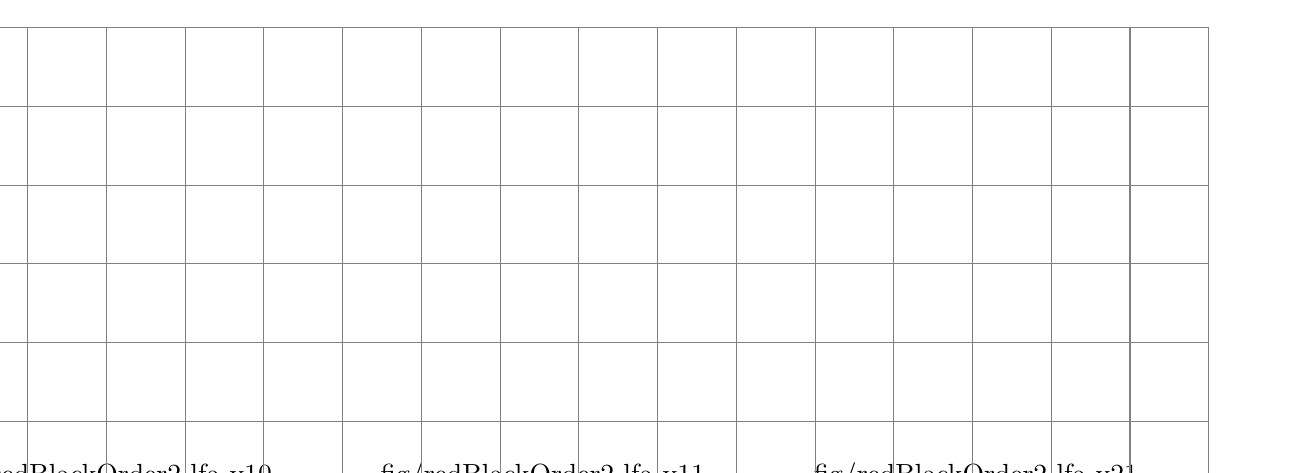
\begin{tikzpicture}[scale=1]
  \useasboundingbox (0,.7) rectangle (16.,6.);  % set the bounding box (so we have less surrounding white space)
%
  \draw (-1.0,0.0) node[anchor=south west,xshift=-4pt,yshift=+0pt] {\trimfig{fig/redBlackOrder2-lfa-v10}{\figWidth}};
  \draw ( 4.5,0.0) node[anchor=south west,xshift=-4pt,yshift=+0pt] {\trimfig{fig/redBlackOrder2-lfa-v11}{\figWidth}};
  \draw (10.0,0.0) node[anchor=south west,xshift=-4pt,yshift=+0pt] {\trimfig{fig/redBlackOrder2-lfa-v21}{\figWidth}};
%
 % \draw (current bounding box.south west) rectangle (current bounding box.north east);
% grid:
 \draw[step=1cm,gray] (-1,0) grid (15,6);
\end{tikzpicture}
\end{center}
\caption{$\omega$-RB-GS results for the second-order accurate discretization with Galerkin coarse grid operator.
The computed smoothing factor $\mu_{\rm opt}$, two-grid and three-grid asymptotic convergence factors,
$\rho_{\rm loc}$ as a function of $\omega$. Shown are results for V[1,0], V[1,1], V[2,1] and V[2,2] cycles.
This figure shows that the optimal value for $\omega$ should not be based on the smoothing factor
when the number of smooths, $\nu_1+\nu_2$, is greater than 1. }
\label{fig:redBlackLFA2}
\end{figure}
}

%\renewcommand{\figWidth}{.475\linewidth}
%\begin{figure}
%\begin{center}
%\epsfig{file=redBlackOrder2.lfa.v10.eps,width=\figWidth}
%\epsfig{file=redBlackOrder2.lfa.v11.eps,width=\figWidth}
%\epsfig{file=redBlackOrder2.lfa.v21.eps,width=\figWidth}
%% \epsfig{file=redBlackOrder2.lfa.v22.eps,width=\figWidth}
%\end{center}
%\caption{$\omega$-RB-GS results for the second-order accurate discretization with Galerkin coarse grid operator.
%The computed smoothing factor $\mu_{\rm opt}$, two-grid and three-grid asymptotic convergence factors,
%$\rho_{\rm loc}$ as a function of $\omega$. Shown are results for V[1,0], V[1,1], V[2,1] and V[2,2] cycles.
%This figure shows that the optimal value for $\omega$ should not be based on the smoothing factor
%when the number of smooths, $\nu_1+\nu_2$, is greater than 1. }
%\label{fig:redBlackLFA2}
%\end{figure}



{
\renewcommand{\figWidth}{6.cm}
\newcommand{\trimfig}[2]{\trimhb{#1}{#2}{.0}{.0}{.0}{.0}}
\begin{figure}[hbt]
\begin{center}
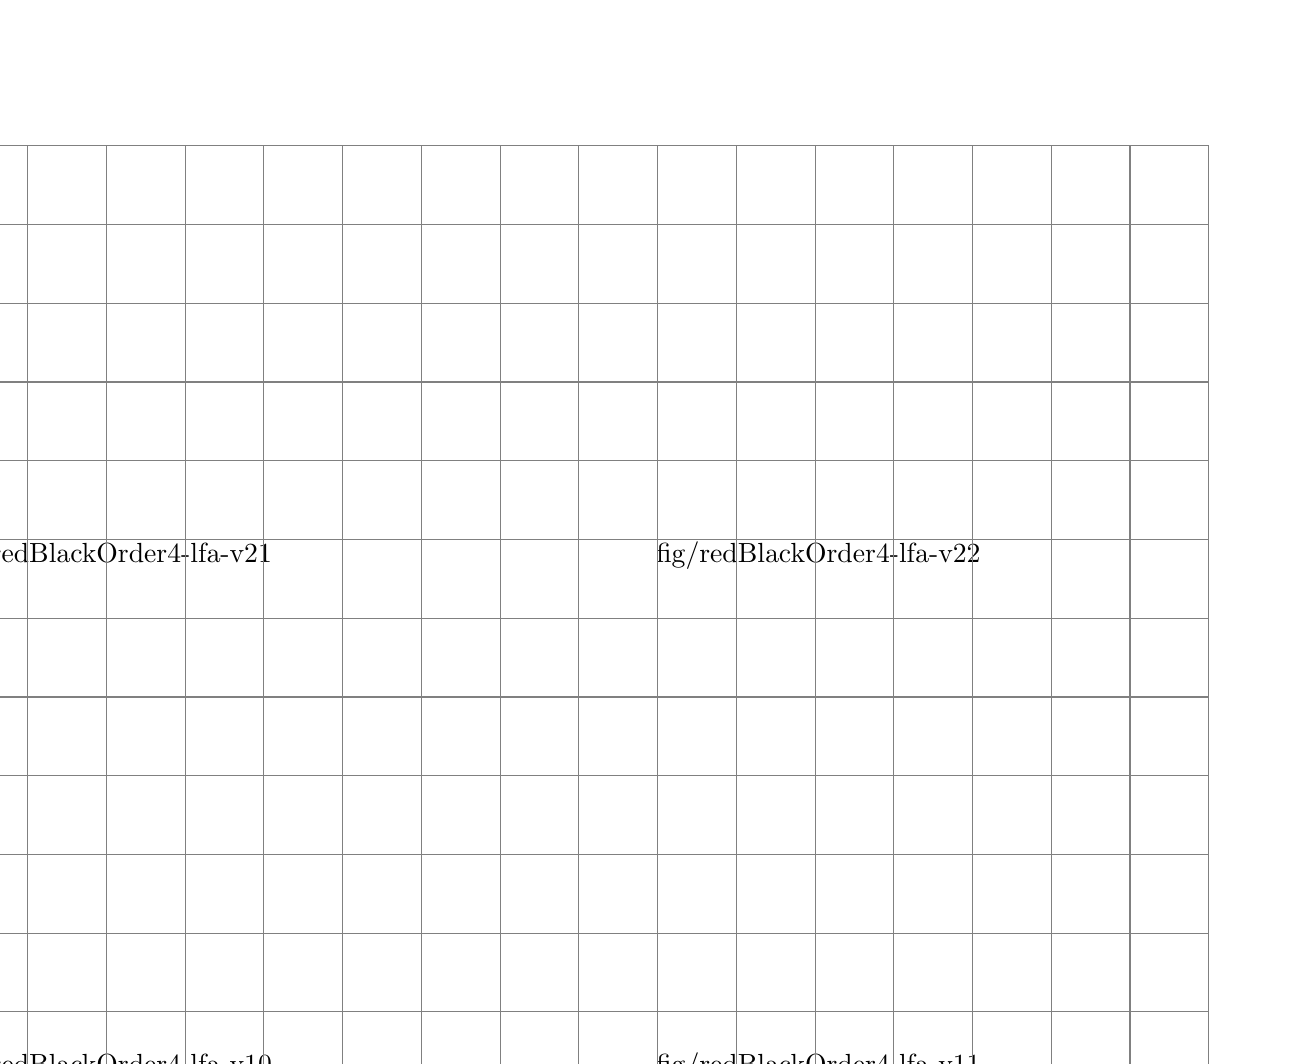
\begin{tikzpicture}[scale=1]
  \useasboundingbox (0,.7) rectangle (16.,13.5);  % set the bounding box (so we have less surrounding white space)
%
  \draw (-1.0,0.0) node[anchor=south west,xshift=-4pt,yshift=+0pt] {\trimfig{fig/redBlackOrder4-lfa-v10}{\figWidth}};
  \draw ( 8.0,0.0) node[anchor=south west,xshift=-4pt,yshift=+0pt] {\trimfig{fig/redBlackOrder4-lfa-v11}{\figWidth}};
  \draw (-1.0,6.5) node[anchor=south west,xshift=-4pt,yshift=+0pt] {\trimfig{fig/redBlackOrder4-lfa-v21}{\figWidth}};
  \draw ( 8.0,6.5) node[anchor=south west,xshift=-4pt,yshift=+0pt] {\trimfig{fig/redBlackOrder4-lfa-v22}{\figWidth}};
%
 % \draw (current bounding box.south west) rectangle (current bounding box.north east);
% grid:
 \draw[step=1cm,gray] (-1,0) grid (15,12);
\end{tikzpicture}
\end{center}
\caption{$\omega$-RB-GS results for the fourth-order accurate discretization.
The computed smoothing factor $\mu_{\rm opt}$, two-grid and three-grid asymptotic convergence factors,
$\rho_{\rm loc}$ as a function of $\omega$. Shown are results for V[1,0], V[1,1], V[2,1] and V[2,2] cycles.
This figure shows that the optimal value for $\omega$ should not be based on the smoothing factor
when the number of smooths, $\nu_1+\nu_2$, is greater than 2. }
\label{fig:redBlackLFA4}
\end{figure}
}



%\renewcommand{\figWidth}{.475\linewidth}
%\begin{figure}
%\begin{center}
%\epsfig{file=redBlackOrder4.lfa.v10.eps,width=\figWidth}
%\epsfig{file=redBlackOrder4.lfa.v11.eps,width=\figWidth}
%\epsfig{file=redBlackOrder4.lfa.v21.eps,width=\figWidth}
%\epsfig{file=redBlackOrder4.lfa.v22.eps,width=\figWidth}
%\end{center}
%\caption{$\omega$-RB-GS results for the fourth-order accurate discretization.
%The computed smoothing factor $\mu_{\rm opt}$, two-grid and three-grid asymptotic convergence factors,
%$\rho_{\rm loc}$ as a function of $\omega$. Shown are results for V[1,0], V[1,1], V[2,1] and V[2,2] cycles.
%This figure shows that the optimal value for $\omega$ should not be based on the smoothing factor
%when the number of smooths, $\nu_1+\nu_2$, is greater than 2. }
%\label{fig:redBlackLFA4}
%\end{figure}


{
\renewcommand{\figWidth}{5.5cm}
\newcommand{\trimfig}[2]{\trimwb{#1}{#2}{.0}{.0}{.0}{.0}}
\begin{figure}[hbt]
\begin{center}
\begin{tikzpicture}[scale=1]
  \useasboundingbox (-.75,.7) rectangle (18.,10);  % set the bounding box (so we have less surrounding white space)
%
  \draw (-1.0,0.0) node[anchor=south west,xshift=-4pt,yshift=+0pt] {\trimfig{fig/redBlackOrder4-lfaOptOmega-v10}{\figWidth}};
  \draw ( 5.0,0.0) node[anchor=south west,xshift=-4pt,yshift=+0pt] {\trimfig{fig/redBlackOrder4-lfaOptMu-v10}{\figWidth}};
  \draw (11.0,0.0) node[anchor=south west,xshift=-4pt,yshift=+0pt] {\trimfig{fig/redBlackOrder4-lfaOptOmega-v11}{\figWidth}};
%                                                                                                              
  \draw (-1.0,5.5) node[anchor=south west,xshift=-4pt,yshift=+0pt] {\trimfig{fig/redBlackOrder4-lfaOptMu-v11}{\figWidth}};
  \draw ( 5.0,5.5) node[anchor=south west,xshift=-4pt,yshift=+0pt] {\trimfig{fig/redBlackOrder4-lfaOptOmega-v21}{\figWidth}};
  \draw (11.0,5.5) node[anchor=south west,xshift=-4pt,yshift=+0pt] {\trimfig{fig/redBlackOrder4-lfaOptMu-v21}{\figWidth}};
%
 % \draw (current bounding box.south west) rectangle (current bounding box.north east);
% grid:
%  \draw[step=1cm,gray] (-1,0) grid (18,11);
\end{tikzpicture}
\end{center}
\caption{$\omega$-RB-GS results for the fourth-order accurate discretization.
The optimal over-relaxation parameter, $\omega_{\rm opt}$, based on the two-grid asymptotic
convergence factor.}
\label{fig:redBlackLFA-2Grid}
\end{figure}
}


%\renewcommand{\figWidth}{.475\linewidth}
%\begin{figure}
%\begin{center}
%\epsfig{file=redBlackOrder4.lfaOptOmega.v10.eps,width=\figWidth}
%\epsfig{file=redBlackOrder4.lfaOptMu.v10.eps,width=\figWidth}
%\epsfig{file=redBlackOrder4.lfaOptOmega.v11.eps,width=\figWidth}
%% 
%\epsfig{file=redBlackOrder4.lfaOptMu.v11.eps,width=\figWidth}
%\epsfig{file=redBlackOrder4.lfaOptOmega.v21.eps,width=\figWidth}
%\epsfig{file=redBlackOrder4.lfaOptMu.v21.eps,width=\figWidth}
%\end{center}
%\caption{$\omega$-RB-GS results for the fourth-order accurate discretization.
%The optimal over-relaxation parameter, $\omega_{\rm opt}$, based on the two-grid asymptotic
%convergence factor.}
%\label{fig:redBlackLFA-2Grid}
%\end{figure}


{
\renewcommand{\figWidth}{7.cm}
\newcommand{\trimfig}[2]{\trimhb{#1}{#2}{.0}{.0}{.0}{.0}}
\begin{figure}[hbt]
\begin{center}
\begin{tikzpicture}[scale=1]
  \useasboundingbox (0,.7) rectangle (16.,7);  % set the bounding box (so we have less surrounding white space)
%
  \draw (-1.0,0.0) node[anchor=south west,xshift=-4pt,yshift=+0pt] {\trimfig{fig/redBlack-order2}{\figWidth}};
%   \draw ( 8.0,0.0) node[anchor=south west,xshift=-4pt,yshift=+0pt] {\trimfig{fig/redBlack-order4-muOpt-nx501}{\figWidth}};
%
 % \draw (current bounding box.south west) rectangle (current bounding box.north east);
% grid:
% \draw[step=1cm,gray] (0,0) grid (15,6);
\end{tikzpicture}
\end{center}
\caption{The optimal over-relaxation parameter, $\omega_{\rm opt}$ and the corresponding smoothing
   rate, $\mu_{\rm opt}$, as a function of ${\rm c}_{\rm min}$. Also shown is the smoothing rate
with $\omega=1$, $\mu(1)$. Left: second-order stencil.
Right: fourth-order stencil. **FIX ME**}
\label{fig:redBlack}
\end{figure}
}



%\renewcommand{\figWidth}{.475\linewidth}
%\begin{figure}
%\begin{center}
%\epsfig{file=redBlack.order2.eps,width=\figWidth}
%% wrong \epsfig{file=redBlack.order4.eps,width=\figWidth}
%\end{center}
%\caption{The optimal over-relaxation parameter, $\omega_{\rm opt}$ and the corresponding smoothing
%   rate, $\mu_{\rm opt}$, as a function of ${\rm c}_{\rm min}$. Also shown is the smoothing rate
%with $\omega=1$, $\mu(1)$. Left: second-order stencil.
%Right: fourth-order stencil.}
%\label{fig:redBlack}
%\end{figure}

{
\renewcommand{\figWidth}{7.cm}
\newcommand{\trimfig}[2]{\trimhb{#1}{#2}{.0}{.0}{.0}{.0}}
\begin{figure}[hbt]
\begin{center}
\begin{tikzpicture}[scale=1]
  \useasboundingbox (0,.7) rectangle (16.,7);  % set the bounding box (so we have less surrounding white space)
%
  \draw (-1.0,0.0) node[anchor=south west,xshift=-4pt,yshift=+0pt] {\trimfig{fig/redBlackSurf-order2}{\figWidth}};
  \draw ( 8.0,0.0) node[anchor=south west,xshift=-4pt,yshift=+0pt] {\trimfig{fig/redBlack-cut-order2}{\figWidth}};
%
 % \draw (current bounding box.south west) rectangle (current bounding box.north east);
% grid:
% \draw[step=1cm,gray] (0,0) grid (15,6);
\end{tikzpicture}
\end{center}
\caption{Smoothing rate as a function of $C=\sum c_i \cos(\theta_i)$ and $\omega$}
\label{fig:redBlackSurf}
\end{figure}
}


%\renewcommand{\figWidth}{.475\linewidth}
%\begin{figure}
%\begin{center}
%\epsfig{file=redBlackSurf.order2.eps,width=\figWidth}
%\epsfig{file=redBlack.cut.order2.eps,width=\figWidth}
%% wrong \epsfig{file=redBlackSurf.order4.eps,width=\figWidth}
%% wrong \epsfig{file=redBlack.cut.order4.eps,width=\figWidth}
%\end{center}
%\caption{Smoothing rate as a function of $C=\sum c_i \cos(\theta_i)$ and $\omega$}
%\label{fig:redBlackSurf}
%\end{figure}




% =============================================================================
\clearpage
\input fourthOrder.tex
% =============================================================================



\clearpage
\section{Numerical Results}\label{sec:numericalResults}

In this section we present some numerical results for some
two and three dimensional problems.

\input notation

% ======================================================================================================
% =================================================================================================
\clearpage
\subsection{Fourth-order accurate circle-in-a-channel}




\begin{figure}[hbt]
\begin{center}
\vglue-.125in
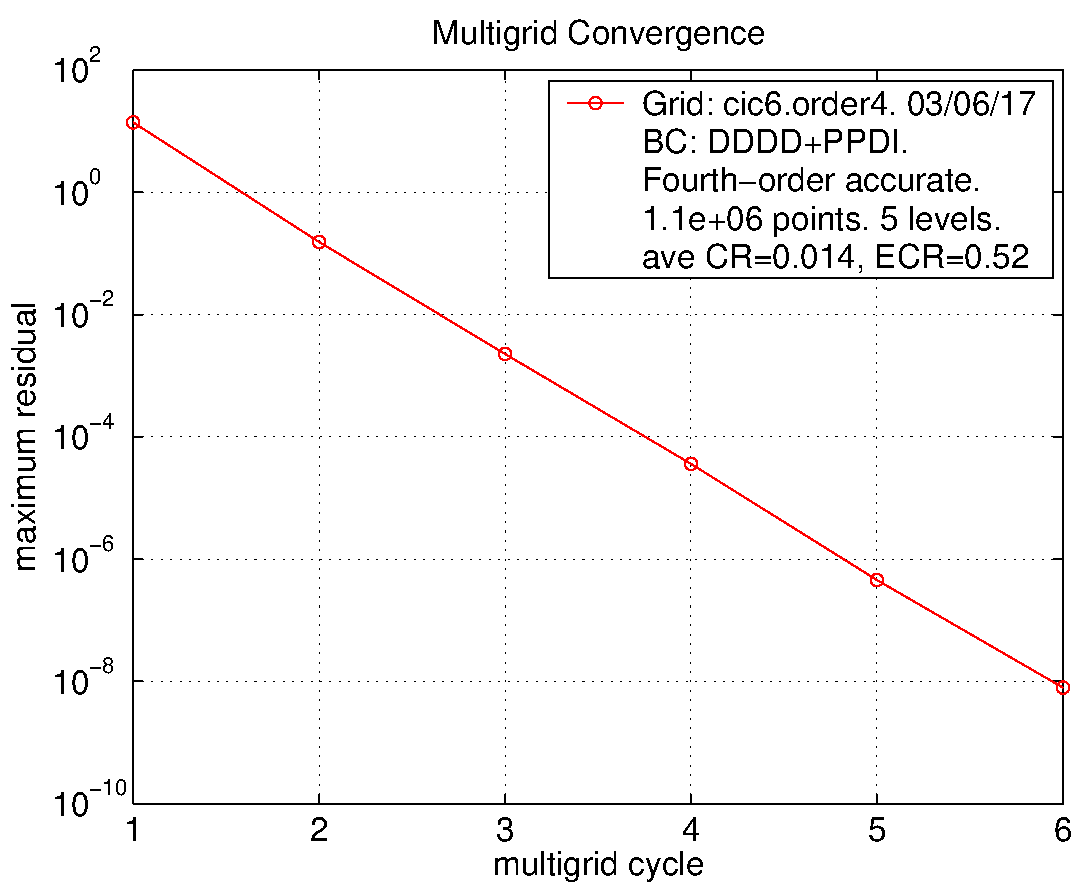
\includegraphics[width=\figWidth]{fig/residual-cic6-order4}
% \epsfig{file=residual.cic6.order4.eps,width=\figWidth}
\end{center}
\caption{Convergence history for a circle-in-a-channel, fourth-order accurate, with IBS smoothing, W[2,1], cic6.order4.}
\label{fig:square1024}
\end{figure}


\begin{figure}[hbt]
\begin{center}
\vglue-.125in
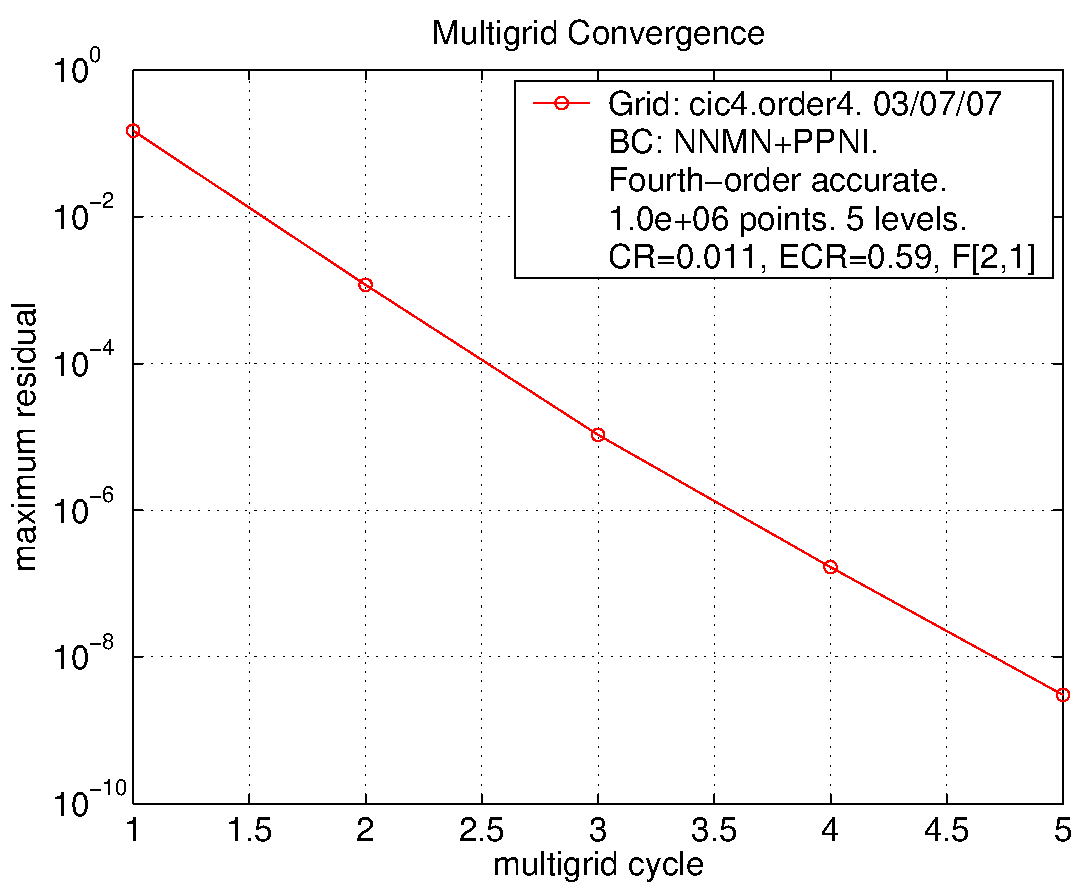
\includegraphics[width=\figWidth]{fig/residual-cic4-mixed-order4}
% \epsfig{file=residual.cic4.mixed.order4.eps,width=\figWidth}
\end{center}
\caption{Convergence history for a circle-in-a-channel, fourth-order accurate with Neumann and mixed boundary
conditions, with IBS smoothing, F[2,1], cic4.order4.}
\label{fig:square1024}
\end{figure}

\subsection{Box}

\renewcommand{\figWidth}{.495\linewidth}
\begin{figure}
\begin{center}
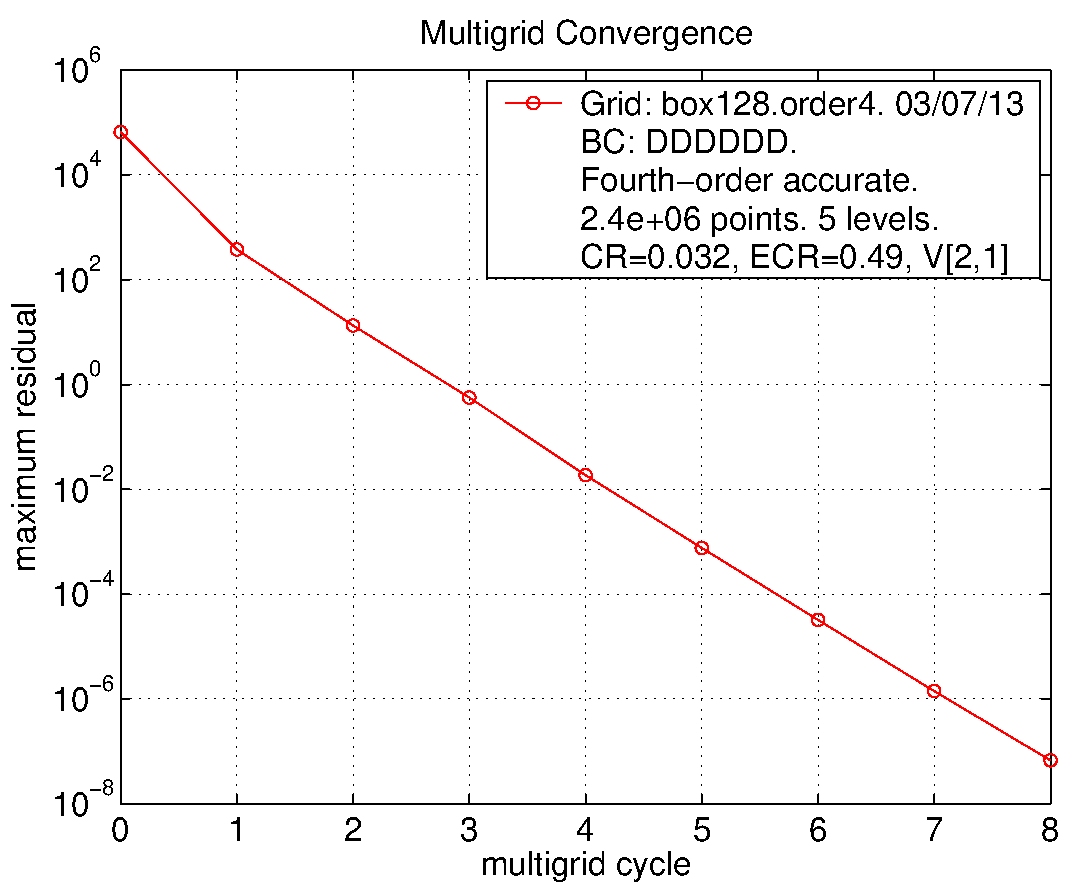
\includegraphics[width=\figWidth]{fig/residual-box128-order4}
% psfig{file=residual.box128.order4.eps,width=\figWidth}
\end{center}
\caption{Convergence history for a box, fourth-order.}
\label{fig:box}
\end{figure}


\subsection{Sphere in a box}

\renewcommand{\figWidth}{.45\linewidth}
\begin{figure}
\begin{center}
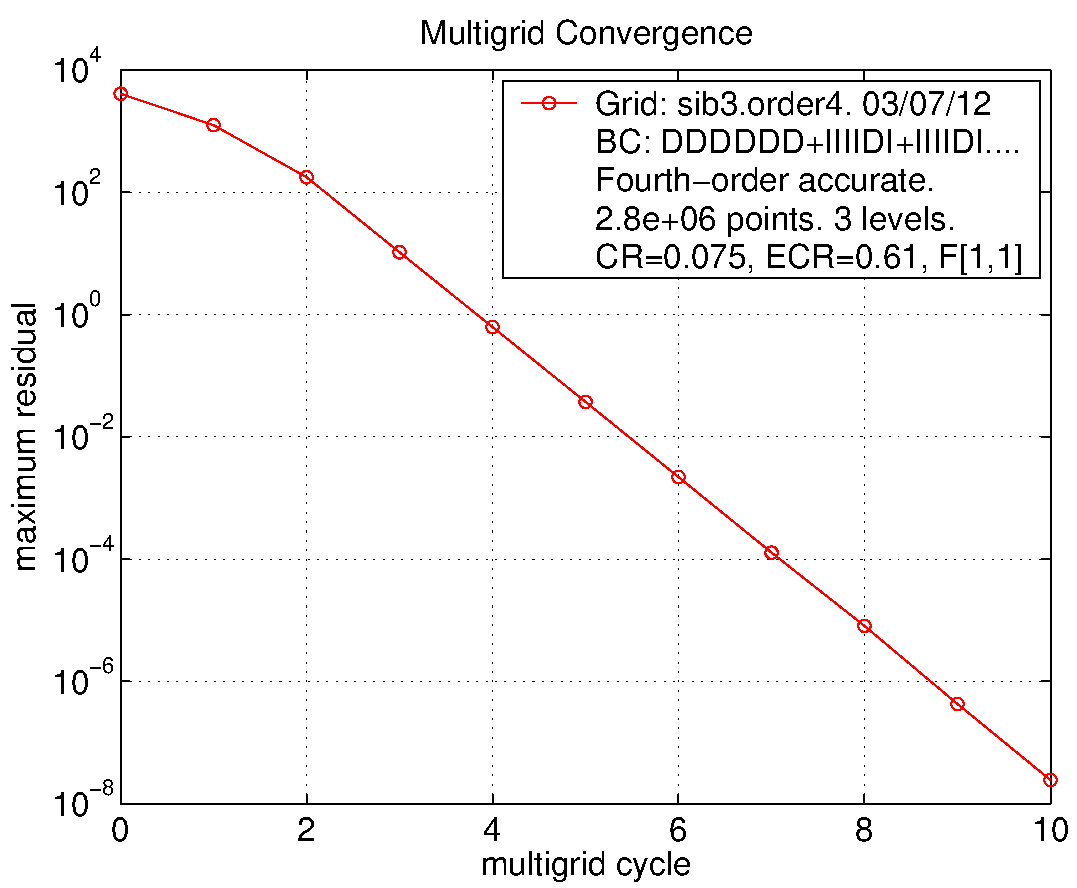
\includegraphics[width=\figWidth]{fig/residual-sib3-order4}
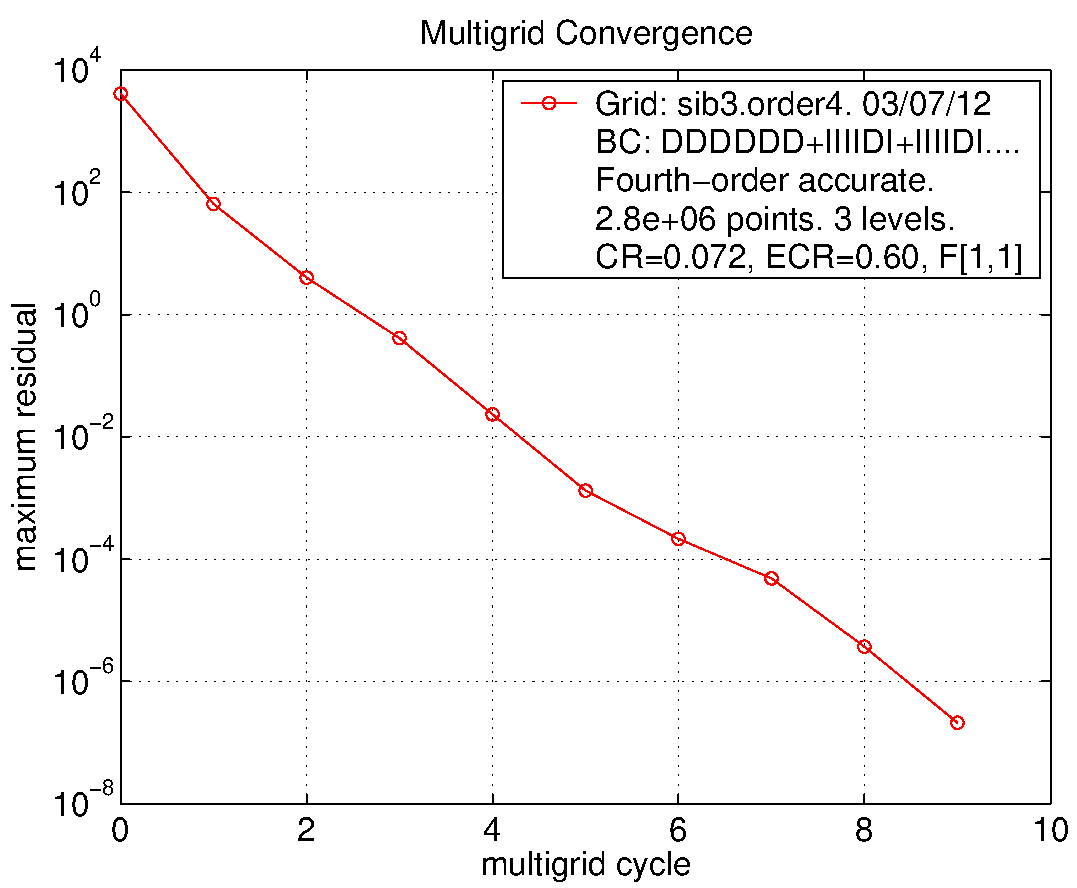
\includegraphics[width=\figWidth]{fig/residual-sib3-order4-fmg}
% \epsfig{file=residual.sib3.order4.eps,width=\figWidth}
% \epsfig{file=residual.sib3.order4.fmg.eps,width=\figWidth}
\end{center}
\caption{Convergence history for a sphere in a box, fourth-order. Right: Full multigrid.}
\label{fig:sib3.order4}
\end{figure}


\begin{figure}
\begin{center}
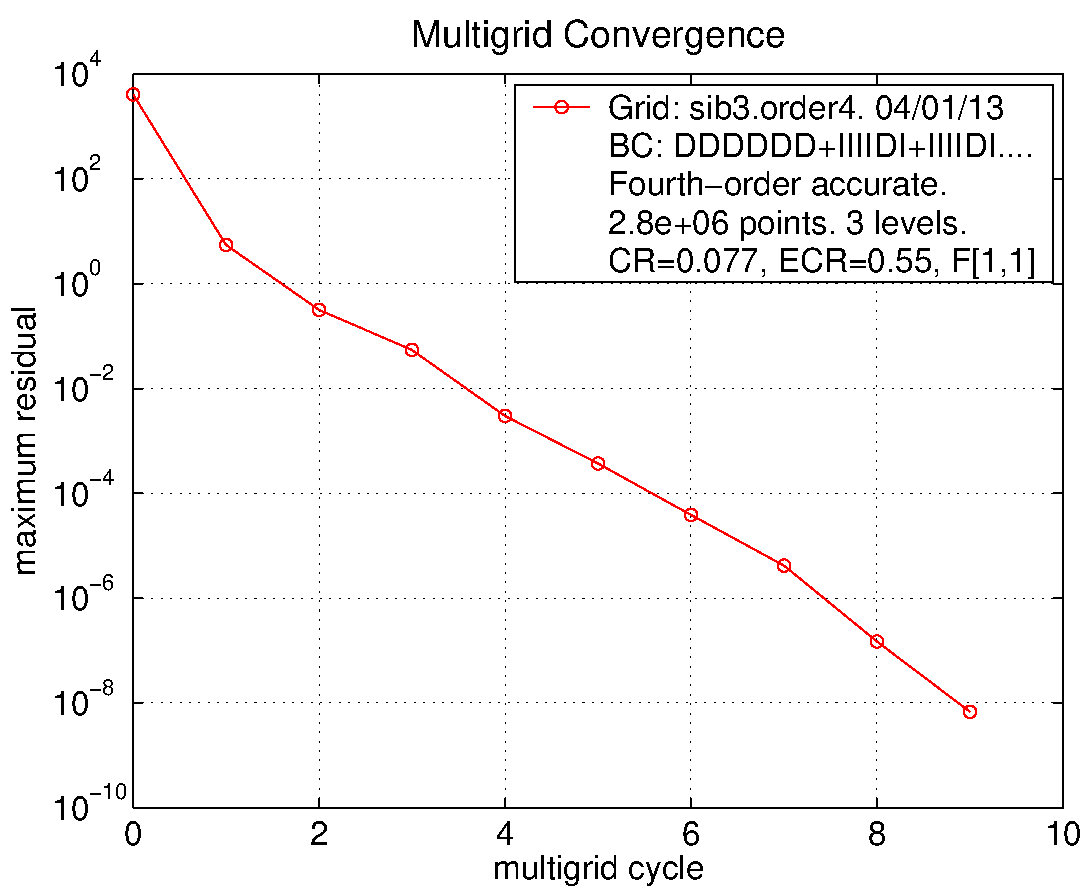
\includegraphics[width=\figWidth]{fig/residual-sib3-order4-F11}
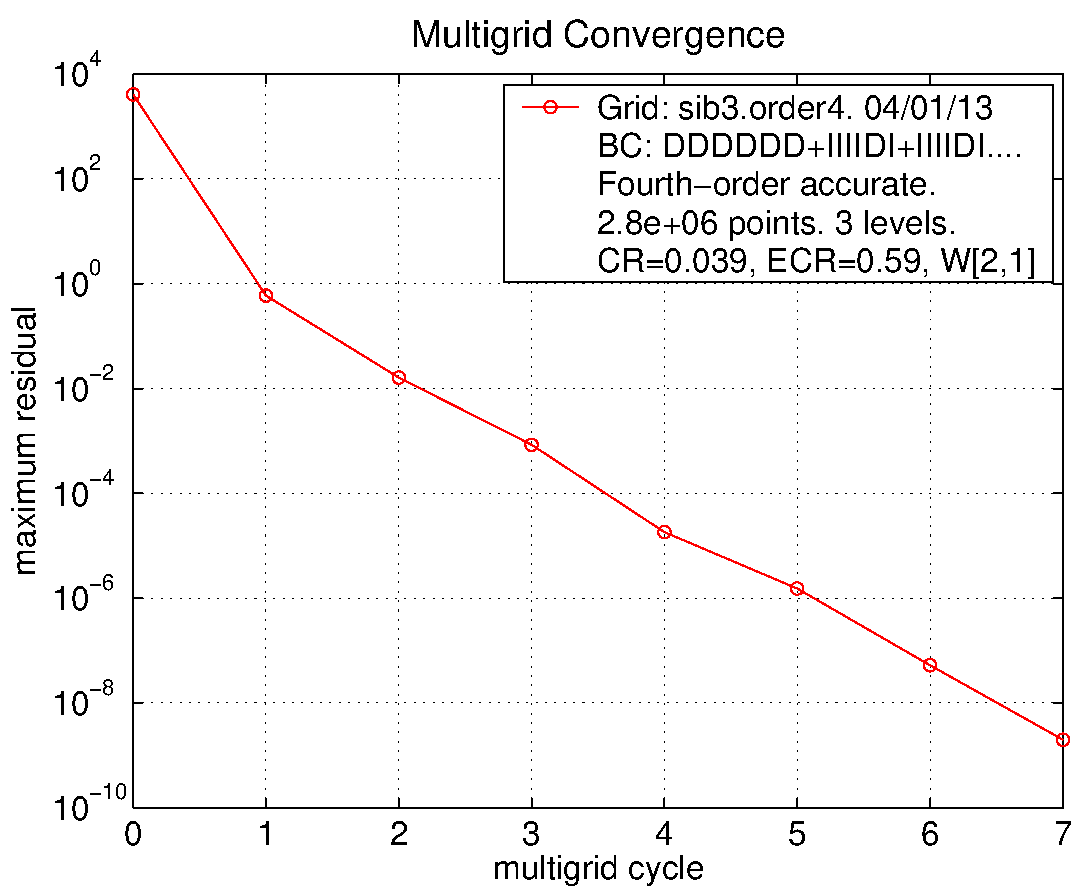
\includegraphics[width=\figWidth]{fig/residual-sib3-order4-W21}
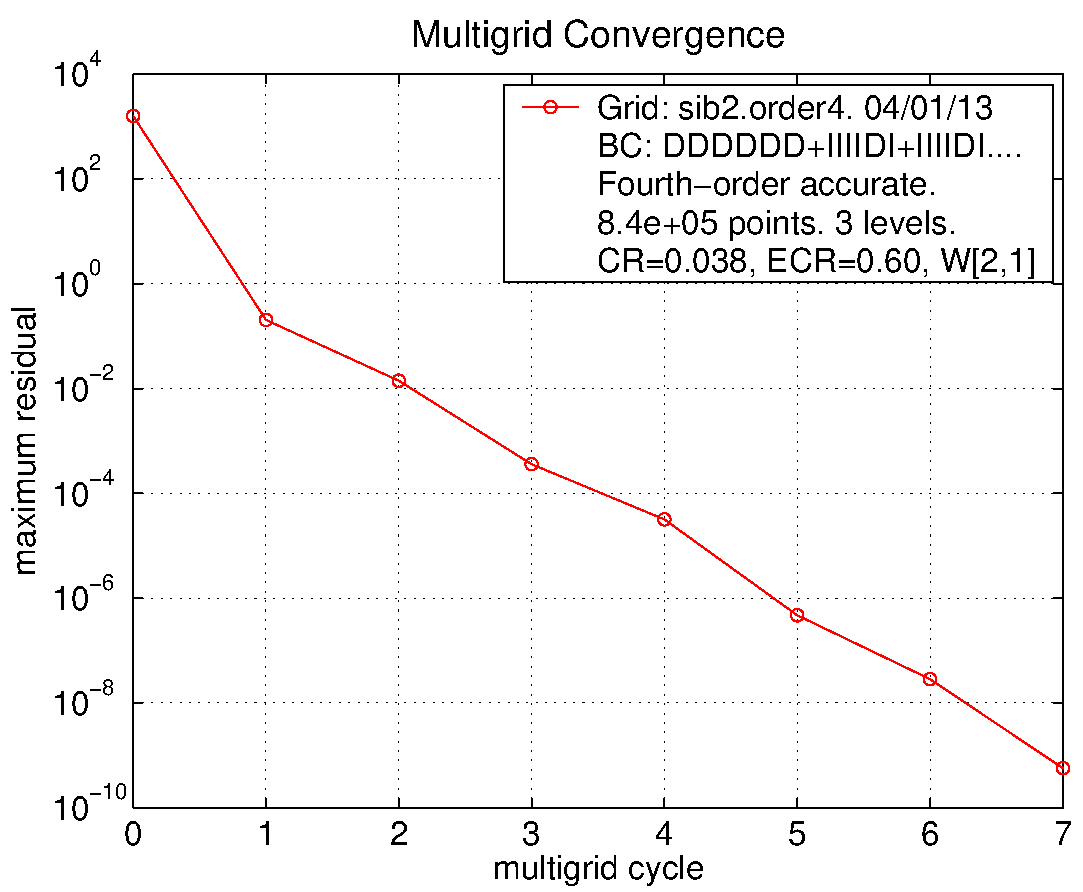
\includegraphics[width=\figWidth]{fig/residual-sib2-order4}
%\epsfig{file=residual.sib3.order4.F11.eps,width=\figWidth}
%\epsfig{file=residual.sib3.order4.W21.eps,width=\figWidth}
%\epsfig{file=residual.sib2.order4.eps,width=\figWidth}
\end{center}
\caption{Convergence history for a sphere in a box, fourth-order. Right: Full multigrid.}
\label{fig:sib3.order4}
\end{figure}

\begin{table}[hbt]
\begin{center}
{\tablefontsize
\begin{tabular}{|c|c|c|c|c|} \hline 
 $i$   & $\vert\vert\mbox{res}\vert\vert_\infty$  &  CR     &  WU    & ECR  \\   \hline 
 $ 1$  & $ 2.5e+00$ & $0.043$ & $ 6.1$ & $0.60$ \\ 
 $ 2$  & $ 1.4e-01$ & $0.056$ & $ 7.5$ & $0.68$ \\ 
 $ 3$  & $ 5.4e-03$ & $0.039$ & $ 8.9$ & $0.69$ \\ 
 $ 4$  & $ 2.1e-04$ & $0.038$ & $ 9.3$ & $0.70$ \\ 
 $ 5$  & $ 2.5e-05$ & $0.120$ & $ 9.3$ & $0.80$ \\ 
 $ 6$  & $ 1.7e-06$ & $0.067$ & $ 9.3$ & $0.75$ \\ 
 $ 7$  & $ 1.1e-07$ & $0.064$ & $ 9.3$ & $0.74$ \\ 
 $ 8$  & $ 5.7e-09$ & $0.053$ & $ 9.3$ & $0.73$ \\ 
\hline 
\multicolumn{5}{|c|}{Grid: sib3.order4. 03/06/18}  \\
\multicolumn{5}{|c|}{BC: DDDDDD+IIIIDI+IIIIDI....}  \\
\multicolumn{5}{|c|}{Fourth-order accurate.}  \\
\multicolumn{5}{|c|}{Trigonometric solution. IBS+PBS}  \\
\multicolumn{5}{|c|}{W[2,1]: rb $\omega=1.20$}  \\
\multicolumn{5}{|c|}{2.78e+06 grid-points. 3 levels.}  \\
\multicolumn{5}{|c|}{Average CR=$0.056$, ECR=$0.72$.}  \\
\multicolumn{5}{|c|}{time/cycle = 2.29e+01 s.}  \\
\hline 
\end{tabular}
\begin{tabular}{|c|c|c|c|c|} \hline 
 $i$   & res      & rate    &  WU    & ECR  \\   \hline 
 $ 1$  & $ 6.0e+01$ & $0.034$ & $ 5.4$ & $0.53$ \\ 
 $ 2$  & $ 2.9e+00$ & $0.048$ & $ 6.8$ & $0.64$ \\ 
 $ 3$  & $ 5.3e-01$ & $0.186$ & $ 8.2$ & $0.81$ \\ 
 $ 4$  & $ 7.5e-02$ & $0.141$ & $ 8.9$ & $0.80$ \\ 
 $ 5$  & $ 9.8e-03$ & $0.131$ & $ 8.9$ & $0.80$ \\ 
 $ 6$  & $ 1.3e-03$ & $0.131$ & $ 8.9$ & $0.80$ \\ 
 $ 7$  & $ 1.7e-04$ & $0.134$ & $ 8.9$ & $0.80$ \\ 
\hline 
\multicolumn{5}{|c|}{Grid: sib3.order4.}  \\
\multicolumn{5}{|c|}{Dirichlet boundary conditions.}  \\
\multicolumn{5}{|c|}{Fourth-order accurate.}  \\
\multicolumn{5}{|c|}{Trigonometric solution.}  \\
\multicolumn{5}{|c|}{Smoother rb[2,1] $\omega=1.20$}  \\
\multicolumn{5}{|c|}{2.78e+06 grid-points. 3 levels.}  \\
\multicolumn{5}{|c|}{Average CR=$0.100$, ECR=$0.75$.}  \\
\multicolumn{5}{|c|}{time/cycle = 1.62e+01 s.}  \\
\hline 
\end{tabular}
} % end \tablefontsize
\end{center}
\caption{Multigrid convergence rates for a sphere-in-a-box, fourth-order accuracy.}
\label{fig:sibII}
\end{table}


\clearpage
\subsection{Performance and Comparison to other methods}

% In table~(\ref{tab:comparison}) we show a comparison of the multigrid solver to an iterative
% solver (stabilized bi-conjugate-gradient from PETSc) and a direct sparse matrix solver (YALE). 

\input comparisonTable

\input performanceTable



\bibliography{\homeHenshaw/papers/common/henshawPapers}
\bibliographystyle{siam}

\printindex

\end{document}




